\documentclass[12pt, twoside]{book} % change to 'oneside' if not printing both sides

%\title{BE(Hons) 2017 thesis template}  % Edit if desired - used by "Overleaf", not currenty used by LaTeX

% The file "Preamble.tex" input here is required to set up the document - keep but edit if required

% =========================================================================
%                        Preamble
% No need to change anything unless you want to add a package.
% =========================================================================

% ESSENTIAL PACKAGES
% -------------------
\usepackage{graphicx}  % essential for inserting any figures
\usepackage[a4paper, left=35mm, right=25mm, top=50mm, bottom=30mm]{geometry}
\usepackage[absolute]{textpos} % required for the "textbox" command used in the title page. (Include option 'showboxes' if you want to see exact location)
   \setlength{\TPHorizModule}{1mm}
   \setlength{\TPVertModule}{1mm}% sets the units to be used for textpos


% SUGGESTED OPTIONAL PACKAGES
% ---------------------------
\usepackage{soul, todonotes}   % good for comments in drafts
\usepackage[authoryear]{natbib}  % recommended, especially for Harvard ref. styles
\usepackage{subfigure, longtable}
\usepackage[colorlinks=true, allcolors=blue]{hyperref}
   % soul & todonotes allow highlighting, comments etc (good for drafts)
   % subfigure allows subfigures (e.g. Fig 1(a) & (b))
   % longtable is handy if you include a nomenclature
   % natbib allows Harvard referencing (with appropriate bibliographystyle)
   % hyperref produces hyperlinks (sometimes clashes with other packages)

   % To include whole pdf pages (with example of use)
%\usepackage{pdfpages}
%\includepdf[pages={1-2}, angle=90, pagecommand={\thispagestyle{plain}}]{BoreBasePlateV2.pdf}

\renewcommand{\bibname}{References}   % Change "Bibliography" to "References"

% If you are using "Overleaf" include this so Overleaf knows what the main file is, otherwise delete this line, it is not used by LaTeX
\title{BE(Hons) 2017 thesis template}

% From https://github.com/goodfeli/dlbook_notation/blob/master/math_commands.tex
%%%%% NEW MATH DEFINITIONS %%%%%

% Mark sections of captions for referring to divisions of figures
\newcommand{\figleft}{{\em (Left)}}
\newcommand{\figcenter}{{\em (Center)}}
\newcommand{\figright}{{\em (Right)}}
\newcommand{\figtop}{{\em (Top)}}
\newcommand{\figbottom}{{\em (Bottom)}}
\newcommand{\captiona}{{\em (a)}}
\newcommand{\captionb}{{\em (b)}}
\newcommand{\captionc}{{\em (c)}}
\newcommand{\captiond}{{\em (d)}}

% Highlight a newly defined term
\newcommand{\newterm}[1]{{\bf #1}}


% Figure reference, lower-case.
\def\figref#1{figure~\ref{#1}}
% Figure reference, capital. For start of sentence
\def\Figref#1{Figure~\ref{#1}}
\def\twofigref#1#2{figures \ref{#1} and \ref{#2}}
\def\quadfigref#1#2#3#4{figures \ref{#1}, \ref{#2}, \ref{#3} and \ref{#4}}
% Section reference, lower-case.
\def\secref#1{section~\ref{#1}}
% Section reference, capital.
\def\Secref#1{Section~\ref{#1}}
% Reference to two sections.
\def\twosecrefs#1#2{sections \ref{#1} and \ref{#2}}
% Reference to three sections.
\def\secrefs#1#2#3{sections \ref{#1}, \ref{#2} and \ref{#3}}
% Reference to an equation, lower-case.
\def\eqref#1{equation~\ref{#1}}
% Reference to an equation, upper case
\def\Eqref#1{Equation~\ref{#1}}
% A raw reference to an equation---avoid using if possible
\def\plaineqref#1{\ref{#1}}
% Reference to a chapter, lower-case.
\def\chapref#1{chapter~\ref{#1}}
% Reference to an equation, upper case.
\def\Chapref#1{Chapter~\ref{#1}}
% Reference to a range of chapters
\def\rangechapref#1#2{chapters\ref{#1}--\ref{#2}}
% Reference to an algorithm, lower-case.
\def\algref#1{algorithm~\ref{#1}}
% Reference to an algorithm, upper case.
\def\Algref#1{Algorithm~\ref{#1}}
\def\twoalgref#1#2{algorithms \ref{#1} and \ref{#2}}
\def\Twoalgref#1#2{Algorithms \ref{#1} and \ref{#2}}
% Reference to a part, lower case
\def\partref#1{part~\ref{#1}}
% Reference to a part, upper case
\def\Partref#1{Part~\ref{#1}}
\def\twopartref#1#2{parts \ref{#1} and \ref{#2}}

\def\ceil#1{\lceil #1 \rceil}
\def\floor#1{\lfloor #1 \rfloor}
\def\1{\bm{1}}
\newcommand{\train}{\mathcal{D}}
\newcommand{\valid}{\mathcal{D_{\mathrm{valid}}}}
\newcommand{\test}{\mathcal{D_{\mathrm{test}}}}

\def\eps{{\epsilon}}


% Random variables
\def\reta{{\textnormal{$\eta$}}}
\def\ra{{\textnormal{a}}}
\def\rb{{\textnormal{b}}}
\def\rc{{\textnormal{c}}}
\def\rd{{\textnormal{d}}}
\def\re{{\textnormal{e}}}
\def\rf{{\textnormal{f}}}
\def\rg{{\textnormal{g}}}
\def\rh{{\textnormal{h}}}
\def\ri{{\textnormal{i}}}
\def\rj{{\textnormal{j}}}
\def\rk{{\textnormal{k}}}
\def\rl{{\textnormal{l}}}
% rm is already a command, just don't name any random variables m
\def\rn{{\textnormal{n}}}
\def\ro{{\textnormal{o}}}
\def\rp{{\textnormal{p}}}
\def\rq{{\textnormal{q}}}
\def\rr{{\textnormal{r}}}
\def\rs{{\textnormal{s}}}
\def\rt{{\textnormal{t}}}
\def\ru{{\textnormal{u}}}
\def\rv{{\textnormal{v}}}
\def\rw{{\textnormal{w}}}
\def\rx{{\textnormal{x}}}
\def\ry{{\textnormal{y}}}
\def\rz{{\textnormal{z}}}

% Random vectors
\def\rvepsilon{{\mathbf{\epsilon}}}
\def\rvtheta{{\mathbf{\theta}}}
\def\rva{{\mathbf{a}}}
\def\rvb{{\mathbf{b}}}
\def\rvc{{\mathbf{c}}}
\def\rvd{{\mathbf{d}}}
\def\rve{{\mathbf{e}}}
\def\rvf{{\mathbf{f}}}
\def\rvg{{\mathbf{g}}}
\def\rvh{{\mathbf{h}}}
\def\rvu{{\mathbf{i}}}
\def\rvj{{\mathbf{j}}}
\def\rvk{{\mathbf{k}}}
\def\rvl{{\mathbf{l}}}
\def\rvm{{\mathbf{m}}}
\def\rvn{{\mathbf{n}}}
\def\rvo{{\mathbf{o}}}
\def\rvp{{\mathbf{p}}}
\def\rvq{{\mathbf{q}}}
\def\rvr{{\mathbf{r}}}
\def\rvs{{\mathbf{s}}}
\def\rvt{{\mathbf{t}}}
\def\rvu{{\mathbf{u}}}
\def\rvv{{\mathbf{v}}}
\def\rvw{{\mathbf{w}}}
\def\rvx{{\mathbf{x}}}
\def\rvy{{\mathbf{y}}}
\def\rvz{{\mathbf{z}}}

% Elements of random vectors
\def\erva{{\textnormal{a}}}
\def\ervb{{\textnormal{b}}}
\def\ervc{{\textnormal{c}}}
\def\ervd{{\textnormal{d}}}
\def\erve{{\textnormal{e}}}
\def\ervf{{\textnormal{f}}}
\def\ervg{{\textnormal{g}}}
\def\ervh{{\textnormal{h}}}
\def\ervi{{\textnormal{i}}}
\def\ervj{{\textnormal{j}}}
\def\ervk{{\textnormal{k}}}
\def\ervl{{\textnormal{l}}}
\def\ervm{{\textnormal{m}}}
\def\ervn{{\textnormal{n}}}
\def\ervo{{\textnormal{o}}}
\def\ervp{{\textnormal{p}}}
\def\ervq{{\textnormal{q}}}
\def\ervr{{\textnormal{r}}}
\def\ervs{{\textnormal{s}}}
\def\ervt{{\textnormal{t}}}
\def\ervu{{\textnormal{u}}}
\def\ervv{{\textnormal{v}}}
\def\ervw{{\textnormal{w}}}
\def\ervx{{\textnormal{x}}}
\def\ervy{{\textnormal{y}}}
\def\ervz{{\textnormal{z}}}

% Random matrices
\def\rmA{{\mathbf{A}}}
\def\rmB{{\mathbf{B}}}
\def\rmC{{\mathbf{C}}}
\def\rmD{{\mathbf{D}}}
\def\rmE{{\mathbf{E}}}
\def\rmF{{\mathbf{F}}}
\def\rmG{{\mathbf{G}}}
\def\rmH{{\mathbf{H}}}
\def\rmI{{\mathbf{I}}}
\def\rmJ{{\mathbf{J}}}
\def\rmK{{\mathbf{K}}}
\def\rmL{{\mathbf{L}}}
\def\rmM{{\mathbf{M}}}
\def\rmN{{\mathbf{N}}}
\def\rmO{{\mathbf{O}}}
\def\rmP{{\mathbf{P}}}
\def\rmQ{{\mathbf{Q}}}
\def\rmR{{\mathbf{R}}}
\def\rmS{{\mathbf{S}}}
\def\rmT{{\mathbf{T}}}
\def\rmU{{\mathbf{U}}}
\def\rmV{{\mathbf{V}}}
\def\rmW{{\mathbf{W}}}
\def\rmX{{\mathbf{X}}}
\def\rmY{{\mathbf{Y}}}
\def\rmZ{{\mathbf{Z}}}

% Elements of random matrices
\def\ermA{{\textnormal{A}}}
\def\ermB{{\textnormal{B}}}
\def\ermC{{\textnormal{C}}}
\def\ermD{{\textnormal{D}}}
\def\ermE{{\textnormal{E}}}
\def\ermF{{\textnormal{F}}}
\def\ermG{{\textnormal{G}}}
\def\ermH{{\textnormal{H}}}
\def\ermI{{\textnormal{I}}}
\def\ermJ{{\textnormal{J}}}
\def\ermK{{\textnormal{K}}}
\def\ermL{{\textnormal{L}}}
\def\ermM{{\textnormal{M}}}
\def\ermN{{\textnormal{N}}}
\def\ermO{{\textnormal{O}}}
\def\ermP{{\textnormal{P}}}
\def\ermQ{{\textnormal{Q}}}
\def\ermR{{\textnormal{R}}}
\def\ermS{{\textnormal{S}}}
\def\ermT{{\textnormal{T}}}
\def\ermU{{\textnormal{U}}}
\def\ermV{{\textnormal{V}}}
\def\ermW{{\textnormal{W}}}
\def\ermX{{\textnormal{X}}}
\def\ermY{{\textnormal{Y}}}
\def\ermZ{{\textnormal{Z}}}

% Vectors
\def\vzero{{\bm{0}}}
\def\vone{{\bm{1}}}
\def\vmu{{\bm{\mu}}}
\def\vtheta{{\bm{\theta}}}
\def\va{{\bm{a}}}
\def\vb{{\bm{b}}}
\def\vc{{\bm{c}}}
\def\vd{{\bm{d}}}
\def\ve{{\bm{e}}}
\def\vf{{\bm{f}}}
\def\vg{{\bm{g}}}
\def\vh{{\bm{h}}}
\def\vi{{\bm{i}}}
\def\vj{{\bm{j}}}
\def\vk{{\bm{k}}}
\def\vl{{\bm{l}}}
\def\vm{{\bm{m}}}
\def\vn{{\bm{n}}}
\def\vo{{\bm{o}}}
\def\vp{{\bm{p}}}
\def\vq{{\bm{q}}}
\def\vr{{\bm{r}}}
\def\vs{{\bm{s}}}
\def\vt{{\bm{t}}}
\def\vu{{\bm{u}}}
\def\vv{{\bm{v}}}
\def\vw{{\bm{w}}}
\def\vx{{\bm{x}}}
\def\vy{{\bm{y}}}
\def\vz{{\bm{z}}}

% Elements of vectors
\def\evalpha{{\alpha}}
\def\evbeta{{\beta}}
\def\evepsilon{{\epsilon}}
\def\evlambda{{\lambda}}
\def\evomega{{\omega}}
\def\evmu{{\mu}}
\def\evpsi{{\psi}}
\def\evsigma{{\sigma}}
\def\evtheta{{\theta}}
\def\eva{{a}}
\def\evb{{b}}
\def\evc{{c}}
\def\evd{{d}}
\def\eve{{e}}
\def\evf{{f}}
\def\evg{{g}}
\def\evh{{h}}
\def\evi{{i}}
\def\evj{{j}}
\def\evk{{k}}
\def\evl{{l}}
\def\evm{{m}}
\def\evn{{n}}
\def\evo{{o}}
\def\evp{{p}}
\def\evq{{q}}
\def\evr{{r}}
\def\evs{{s}}
\def\evt{{t}}
\def\evu{{u}}
\def\evv{{v}}
\def\evw{{w}}
\def\evx{{x}}
\def\evy{{y}}
\def\evz{{z}}

% Matrix
\def\mA{{\bm{A}}}
\def\mB{{\bm{B}}}
\def\mC{{\bm{C}}}
\def\mD{{\bm{D}}}
\def\mE{{\bm{E}}}
\def\mF{{\bm{F}}}
\def\mG{{\bm{G}}}
\def\mH{{\bm{H}}}
\def\mI{{\bm{I}}}
\def\mJ{{\bm{J}}}
\def\mK{{\bm{K}}}
\def\mL{{\bm{L}}}
\def\mM{{\bm{M}}}
\def\mN{{\bm{N}}}
\def\mO{{\bm{O}}}
\def\mP{{\bm{P}}}
\def\mQ{{\bm{Q}}}
\def\mR{{\bm{R}}}
\def\mS{{\bm{S}}}
\def\mT{{\bm{T}}}
\def\mU{{\bm{U}}}
\def\mV{{\bm{V}}}
\def\mW{{\bm{W}}}
\def\mX{{\bm{X}}}
\def\mY{{\bm{Y}}}
\def\mZ{{\bm{Z}}}
\def\mBeta{{\bm{\beta}}}
\def\mPhi{{\bm{\Phi}}}
\def\mLambda{{\bm{\Lambda}}}
\def\mSigma{{\bm{\Sigma}}}

% Tensor
\DeclareMathAlphabet{\mathsfit}{\encodingdefault}{\sfdefault}{m}{sl}
\SetMathAlphabet{\mathsfit}{bold}{\encodingdefault}{\sfdefault}{bx}{n}
\newcommand{\tens}[1]{\bm{\mathsfit{#1}}}
\def\tA{{\tens{A}}}
\def\tB{{\tens{B}}}
\def\tC{{\tens{C}}}
\def\tD{{\tens{D}}}
\def\tE{{\tens{E}}}
\def\tF{{\tens{F}}}
\def\tG{{\tens{G}}}
\def\tH{{\tens{H}}}
\def\tI{{\tens{I}}}
\def\tJ{{\tens{J}}}
\def\tK{{\tens{K}}}
\def\tL{{\tens{L}}}
\def\tM{{\tens{M}}}
\def\tN{{\tens{N}}}
\def\tO{{\tens{O}}}
\def\tP{{\tens{P}}}
\def\tQ{{\tens{Q}}}
\def\tR{{\tens{R}}}
\def\tS{{\tens{S}}}
\def\tT{{\tens{T}}}
\def\tU{{\tens{U}}}
\def\tV{{\tens{V}}}
\def\tW{{\tens{W}}}
\def\tX{{\tens{X}}}
\def\tY{{\tens{Y}}}
\def\tZ{{\tens{Z}}}


% Graph
\def\gA{{\mathcal{A}}}
\def\gB{{\mathcal{B}}}
\def\gC{{\mathcal{C}}}
\def\gD{{\mathcal{D}}}
\def\gE{{\mathcal{E}}}
\def\gF{{\mathcal{F}}}
\def\gG{{\mathcal{G}}}
\def\gH{{\mathcal{H}}}
\def\gI{{\mathcal{I}}}
\def\gJ{{\mathcal{J}}}
\def\gK{{\mathcal{K}}}
\def\gL{{\mathcal{L}}}
\def\gM{{\mathcal{M}}}
\def\gN{{\mathcal{N}}}
\def\gO{{\mathcal{O}}}
\def\gP{{\mathcal{P}}}
\def\gQ{{\mathcal{Q}}}
\def\gR{{\mathcal{R}}}
\def\gS{{\mathcal{S}}}
\def\gT{{\mathcal{T}}}
\def\gU{{\mathcal{U}}}
\def\gV{{\mathcal{V}}}
\def\gW{{\mathcal{W}}}
\def\gX{{\mathcal{X}}}
\def\gY{{\mathcal{Y}}}
\def\gZ{{\mathcal{Z}}}

% Sets
\def\sA{{\mathbb{A}}}
\def\sB{{\mathbb{B}}}
\def\sC{{\mathbb{C}}}
\def\sD{{\mathbb{D}}}
% Don't use a set called E, because this would be the same as our symbol
% for expectation.
\def\sF{{\mathbb{F}}}
\def\sG{{\mathbb{G}}}
\def\sH{{\mathbb{H}}}
\def\sI{{\mathbb{I}}}
\def\sJ{{\mathbb{J}}}
\def\sK{{\mathbb{K}}}
\def\sL{{\mathbb{L}}}
\def\sM{{\mathbb{M}}}
\def\sN{{\mathbb{N}}}
\def\sO{{\mathbb{O}}}
\def\sP{{\mathbb{P}}}
\def\sQ{{\mathbb{Q}}}
\def\sR{{\mathbb{R}}}
\def\sS{{\mathbb{S}}}
\def\sT{{\mathbb{T}}}
\def\sU{{\mathbb{U}}}
\def\sV{{\mathbb{V}}}
\def\sW{{\mathbb{W}}}
\def\sX{{\mathbb{X}}}
\def\sY{{\mathbb{Y}}}
\def\sZ{{\mathbb{Z}}}

% Entries of a matrix
\def\emLambda{{\Lambda}}
\def\emA{{A}}
\def\emB{{B}}
\def\emC{{C}}
\def\emD{{D}}
\def\emE{{E}}
\def\emF{{F}}
\def\emG{{G}}
\def\emH{{H}}
\def\emI{{I}}
\def\emJ{{J}}
\def\emK{{K}}
\def\emL{{L}}
\def\emM{{M}}
\def\emN{{N}}
\def\emO{{O}}
\def\emP{{P}}
\def\emQ{{Q}}
\def\emR{{R}}
\def\emS{{S}}
\def\emT{{T}}
\def\emU{{U}}
\def\emV{{V}}
\def\emW{{W}}
\def\emX{{X}}
\def\emY{{Y}}
\def\emZ{{Z}}
\def\emSigma{{\Sigma}}

% entries of a tensor
% Same font as tensor, without \bm wrapper
\newcommand{\etens}[1]{\mathsfit{#1}}
\def\etLambda{{\etens{\Lambda}}}
\def\etA{{\etens{A}}}
\def\etB{{\etens{B}}}
\def\etC{{\etens{C}}}
\def\etD{{\etens{D}}}
\def\etE{{\etens{E}}}
\def\etF{{\etens{F}}}
\def\etG{{\etens{G}}}
\def\etH{{\etens{H}}}
\def\etI{{\etens{I}}}
\def\etJ{{\etens{J}}}
\def\etK{{\etens{K}}}
\def\etL{{\etens{L}}}
\def\etM{{\etens{M}}}
\def\etN{{\etens{N}}}
\def\etO{{\etens{O}}}
\def\etP{{\etens{P}}}
\def\etQ{{\etens{Q}}}
\def\etR{{\etens{R}}}
\def\etS{{\etens{S}}}
\def\etT{{\etens{T}}}
\def\etU{{\etens{U}}}
\def\etV{{\etens{V}}}
\def\etW{{\etens{W}}}
\def\etX{{\etens{X}}}
\def\etY{{\etens{Y}}}
\def\etZ{{\etens{Z}}}

% The true underlying data generating distribution
\newcommand{\pdata}{p_{\rm{data}}}
% The empirical distribution defined by the training set
\newcommand{\ptrain}{\hat{p}_{\rm{data}}}
\newcommand{\Ptrain}{\hat{P}_{\rm{data}}}
% The model distribution
\newcommand{\pmodel}{p_{\rm{model}}}
\newcommand{\Pmodel}{P_{\rm{model}}}
\newcommand{\ptildemodel}{\tilde{p}_{\rm{model}}}
% Stochastic autoencoder distributions
\newcommand{\pencode}{p_{\rm{encoder}}}
\newcommand{\pdecode}{p_{\rm{decoder}}}
\newcommand{\precons}{p_{\rm{reconstruct}}}

\newcommand{\laplace}{\mathrm{Laplace}} % Laplace distribution

\newcommand{\E}{\mathbb{E}}
\newcommand{\Ls}{\mathcal{L}}
\newcommand{\R}{\mathbb{R}}
\newcommand{\emp}{\tilde{p}}
\newcommand{\lr}{\alpha}
\newcommand{\reg}{\lambda}
\newcommand{\rect}{\mathrm{rectifier}}
\newcommand{\softmax}{\mathrm{softmax}}
\newcommand{\sigmoid}{\sigma}
\newcommand{\softplus}{\zeta}
\newcommand{\KL}{D_{\mathrm{KL}}}
\newcommand{\Var}{\mathrm{Var}}
\newcommand{\standarderror}{\mathrm{SE}}
\newcommand{\Cov}{\mathrm{Cov}}
% Wolfram Mathworld says $L^2$ is for function spaces and $\ell^2$ is for vectors
% But then they seem to use $L^2$ for vectors throughout the site, and so does
% wikipedia.
\newcommand{\normlzero}{L^0}
\newcommand{\normlone}{L^1}
\newcommand{\normltwo}{L^2}
\newcommand{\normlp}{L^p}
\newcommand{\normmax}{L^\infty}

\newcommand{\parents}{Pa} % See usage in notation.tex. Chosen to match Daphne's book.

\DeclareMathOperator*{\argmax}{arg\,max}
\DeclareMathOperator*{\argmin}{arg\,min}

\DeclareMathOperator{\sign}{sign}
\DeclareMathOperator{\Tr}{Tr}
\let\ab\allowbreak

\begin{document}

% =========================================================================
%                        Front matter 
%   Modify cover page, declaration, abstract, acknowledgements, Nomenclature
%   etc. as required. For draft purposes you can comment out some lines.
% =========================================================================
\frontmatter                % Don't delete this line

\cleardoublepage

\thispagestyle{empty} % suppress header/footer for the title page
%      1.   Title page
%---------------------------
% May need to adjust dimensions: currently 120x55 @ (45,53) from top left of page (in mm)
\begin{textblock}{120}(45,53) % {width}(x,y) top-left rel to page top-left
\noindent\begin{minipage}[t][55mm][c]{\textwidth} 
\centering \Large  % change to '\large' if it doesn't fit
\vspace*{\fill}
{\bf UTas BE(Hons) Thesis Template:\\ with a title that takes up two lines or more}
\vfill
A.U. Thor, 123456 
\vfill
\large October 2017
\vspace*{\fill}
\end{minipage}
\end{textblock}

% Optional: University of Tasmania Logo
\begin{textblock}{120}(45,155)
\centering
\begin{figure}[h]
\centering
\includegraphics[width=0.75\linewidth]{UTAS-Logo-colour.eps}
\end{figure}
\vspace{2cm}
\Large
School of Engineering and ICT


\end{textblock}


% Footer of title page - edit only if you are doing BSc-BE(Hons)
% --------------------------------------------------------------
\begin{textblock}{150}(30,250)
\centering
\emph{This thesis is submitted in partial fulfilment of the requirements for the degree of
%Bachelor of Science and   %% uncomment this line if doing BSc-BE(Hons)
Bachelor of Engineering with Honours,
University of Tasmania.}
\end{textblock}



% suppress page numbering until declaration page
\pagenumbering{gobble}
\null\cleardoublepage
\pagenumbering{roman}


%      2.   Declaration
%---------------------------
\chapter{Declaration}

This Thesis to the best of my knowledge and belief contains no material published or unpublished that was written by another person, nor any material that infringes copyright, nor any material that has been accepted for a degree or diploma by University of Tasmania or any other institution, except by way of background information and where due acknowledgement is made in the text of the Thesis.

This Thesis is the result of my own investigations, except where otherwise stated. Other sources are acknowledged in the text giving explicit references. A list of references is appended.

% select one of the following paragraphs, modify if necessary

I hereby give consent for my Thesis to be available for photocopying, inter-library loan, electronic access to University of Tasmania staff and students via the University of Tasmania library, and for the title and summary to be made available to outside organisations, in accordance with the Copyright Act 1968.

%This thesis is not to be made available for loan or copying for [{\em insert period of time}] following the date of this statement. Following that time the thesis may be made available for loan and limited copying in accordance with the Copyright Act 1968.

   \bigskip
   \bigskip

Signed:

   \bigskip
   \bigskip

Dated: \hl{ 1st May 2018 }      % replace with an actual date if you don't want today's date
%      3.   Abstract
%---------------------------

\chapter{Abstract}

\hl{Insert your abstract here.}
%      4.   Acknowledgements
%---------------------------
\chapter{Acknowledgements}

People to thank are\ldots \hl{(insert your acknowledgements)}
\tableofcontents
\listoffigures   % optional
\listoftables    % optional
%      6.   Nomenclature (optional)
%---------------------------
\chapter{Nomenclature}
Notation below is reproduced from \citet{Goodfellow-et-al-2016}.

% From https://github.com/goodfeli/dlbook_notation/blob/master/notation.tex

\vspace{\notationgap}
% Need to use minipage to keep title of table on same page as table
\begin{minipage}{\textwidth}
	% This is a hack to put a little title over the table
	% We cannot use "\section*", etc., they appear in the table of contents.
	% tocdepth does not work on this chapter.
	\centerline{\bf Numbers and Arrays}
	\bgroup
	% The \arraystretch definition here increases the space between rows in the table,
	% so that \displaystyle math has more vertical space.
	\def\arraystretch{1.5}
	\begin{tabular}{cp{3.25in}}
		$\displaystyle a$ & A scalar (integer or real)\\
		$\displaystyle \va$ & A vector\\
		$\displaystyle \mA$ & A matrix\\
		$\displaystyle \tA$ & A tensor\\
		$\displaystyle \mI_n$ & Identity matrix with $n$ rows and $n$ columns\\
		$\displaystyle \mI$ & Identity matrix with dimensionality implied by context\\
		$\displaystyle \ve^{(i)}$ & Standard basis vector $[0,\dots,0,1,0,\dots,0]$ with a 1 at position $i$\\
		$\displaystyle \text{diag}(\va)$ & A square, diagonal matrix with diagonal entries given by $\va$\\
		$\displaystyle \ra$ & A scalar random variable\\
		$\displaystyle \rva$ & A vector-valued random variable\\
		$\displaystyle \rmA$ & A matrix-valued random variable\\
	\end{tabular}
	\egroup
	\index{Scalar}
	\index{Vector}
	\index{Matrix}
	\index{Tensor}
\end{minipage}

\vspace{\notationgap}
\begin{minipage}{\textwidth}
	\centerline{\bf Sets and Graphs}
	\bgroup
	\def\arraystretch{1.5}
	\begin{tabular}{cp{3.25in}}
		$\displaystyle \sA$ & A set\\
		$\displaystyle \R$ & The set of real numbers \\
		% NOTE: do not use \R^+, because it is ambiguous whether:
		% - It includes 0
		% - It includes only real numbers, or also infinity.
		% We usually do not include infinity, so we may explicitly write
		% [0, \infty) to include 0
		% (0, \infty) to not include 0
		$\displaystyle \{0, 1\}$ & The set containing 0 and 1 \\
		$\displaystyle \{0, 1, \dots, n \}$ & The set of all integers between $0$ and $n$\\
		$\displaystyle [a, b]$ & The real interval including $a$ and $b$\\
		$\displaystyle (a, b]$ & The real interval excluding $a$ but including $b$\\
		$\displaystyle \sA \backslash \sB$ & Set subtraction, i.e., the set containing the elements of $\sA$ that are not in $\sB$\\
		$\displaystyle \gG$ & A graph\\
		$\displaystyle \parents_\gG(\ervx_i)$ & The parents of $\ervx_i$ in $\gG$
	\end{tabular}
	\egroup
	\index{Scalar}
	\index{Vector}
	\index{Matrix}
	\index{Tensor}
	\index{Graph}
	\index{Set}
\end{minipage}

\vspace{\notationgap}
\begin{minipage}{\textwidth}
	\centerline{\bf Indexing}
	\bgroup
	\def\arraystretch{1.5}
	\begin{tabular}{cp{3.25in}}
		$\displaystyle \eva_i$ & Element $i$ of vector $\va$, with indexing starting at 1 \\
		$\displaystyle \eva_{-i}$ & All elements of vector $\va$ except for element $i$ \\
		$\displaystyle \emA_{i,j}$ & Element $i, j$ of matrix $\mA$ \\
		$\displaystyle \mA_{i, :}$ & Row $i$ of matrix $\mA$ \\
		$\displaystyle \mA_{:, i}$ & Column $i$ of matrix $\mA$ \\
		$\displaystyle \etA_{i, j, k}$ & Element $(i, j, k)$ of a 3-D tensor $\tA$\\
		$\displaystyle \tA_{:, :, i}$ & 2-D slice of a 3-D tensor\\
		$\displaystyle \erva_i$ & Element $i$ of the random vector $\rva$ \\
	\end{tabular}
	\egroup
\end{minipage}

\vspace{\notationgap}
\begin{minipage}{\textwidth}
	\centerline{\bf Linear Algebra Operations}
	\bgroup
	\def\arraystretch{1.5}
	\begin{tabular}{cp{3.25in}}
		$\displaystyle \mA^\top$ & Transpose of matrix $\mA$ \\
		$\displaystyle \mA^+$ & Moore-Penrose pseudoinverse of $\mA$\\
		$\displaystyle \mA \odot \mB $ & Element-wise (Hadamard) product of $\mA$ and $\mB$ \\
		% Wikipedia uses \circ for element-wise multiplication but this could be confused with function composition
		$\displaystyle \mathrm{det}(\mA)$ & Determinant of $\mA$ \\
	\end{tabular}
	\egroup
	\index{Transpose}
	\index{Element-wise product|see {Hadamard product}}
	\index{Hadamard product}
	\index{Determinant}
\end{minipage}

\vspace{\notationgap}
\begin{minipage}{\textwidth}
	\centerline{\bf Calculus}
	\bgroup
	\def\arraystretch{1.5}
	\begin{tabular}{cp{3.25in}}
		% NOTE: the [2ex] on the next line adds extra height to that row of the table.
		% Without that command, the fraction on the first line is too tall and collides
		% with the fraction on the second line.
		$\displaystyle\frac{d y} {d x}$ & Derivative of $y$ with respect to $x$\\ [2ex]
		$\displaystyle \frac{\partial y} {\partial x} $ & Partial derivative of $y$ with respect to $x$ \\
		$\displaystyle \nabla_\vx y $ & Gradient of $y$ with respect to $\vx$ \\
		$\displaystyle \nabla_\mX y $ & Matrix derivatives of $y$ with respect to $\mX$ \\
		$\displaystyle \nabla_\tX y $ & Tensor containing derivatives of $y$ with respect to $\tX$ \\
		$\displaystyle \frac{\partial f}{\partial \vx} $ & Jacobian matrix $\mJ \in \R^{m\times n}$ of $f: \R^n \rightarrow \R^m$\\
		$\displaystyle \nabla_\vx^2 f(\vx)\text{ or }\mH( f)(\vx)$ & The Hessian matrix of $f$ at input point $\vx$\\
		$\displaystyle \int f(\vx) d\vx $ & Definite integral over the entire domain of $\vx$ \\
		$\displaystyle \int_\sS f(\vx) d\vx$ & Definite integral with respect to $\vx$ over the set $\sS$ \\
	\end{tabular}
	\egroup
	\index{Derivative}
	\index{Integral}
	\index{Jacobian matrix}
	\index{Hessian matrix}
\end{minipage}

\vspace{\notationgap}
\begin{minipage}{\textwidth}
	\centerline{\bf Probability and Information Theory}
	\bgroup
	\def\arraystretch{1.5}
	\begin{tabular}{cp{3.25in}}
		$\displaystyle \ra \bot \rb$ & The random variables $\ra$ and $\rb$ are independent\\
		$\displaystyle \ra \bot \rb \mid \rc $ & They are conditionally independent given $\rc$\\
		$\displaystyle P(\ra)$ & A probability distribution over a discrete variable\\
		$\displaystyle p(\ra)$ & A probability distribution over a continuous variable, or over
		a variable whose type has not been specified\\
		$\displaystyle \ra \sim P$ & Random variable $\ra$ has distribution $P$\\% so thing on left of \sim should always be a random variable, with name beginning with \r
		$\displaystyle  \E_{\rx\sim P} [ f(x) ]\text{ or } \E f(x)$ & Expectation of $f(x)$ with respect to $P(\rx)$ \\
		$\displaystyle \Var(f(x)) $ &  Variance of $f(x)$ under $P(\rx)$ \\
		$\displaystyle \Cov(f(x),g(x)) $ & Covariance of $f(x)$ and $g(x)$ under $P(\rx)$\\
		$\displaystyle H(\rx) $ & Shannon entropy of the random variable $\rx$\\
		$\displaystyle \KL ( P \Vert Q ) $ & Kullback-Leibler divergence of P and Q \\
		$\displaystyle \mathcal{N} ( \vx ; \vmu , \mSigma)$ & Gaussian distribution %
		over $\vx$ with mean $\vmu$ and covariance $\mSigma$ \\
	\end{tabular}
	\egroup
	\index{Independence}
	\index{Conditional independence}
	\index{Variance}
	\index{Covariance}
	\index{Kullback-Leibler divergence}
	\index{Shannon entropy}
\end{minipage}

\vspace{\notationgap}
\begin{minipage}{\textwidth}
	\centerline{\bf Functions}
	\bgroup
	\def\arraystretch{1.5}
	\begin{tabular}{cp{3.25in}}
		$\displaystyle f: \sA \rightarrow \sB$ & The function $f$ with domain $\sA$ and range $\sB$\\
		$\displaystyle f \circ g $ & Composition of the functions $f$ and $g$ \\
		$\displaystyle f(\vx ; \vtheta) $ & A function of $\vx$ parametrized by $\vtheta$.
		(Sometimes we write $f(\vx)$ and omit the argument $\vtheta$ to lighten notation) \\
		$\displaystyle \log x$ & Natural logarithm of $x$ \\
		$\displaystyle \sigma(x)$ & Logistic sigmoid, $\displaystyle \frac{1} {1 + \exp(-x)}$ \\
		$\displaystyle \zeta(x)$ & Softplus, $\log(1 + \exp(x))$ \\
		$\displaystyle || \vx ||_p $ & $\normlp$ norm of $\vx$ \\
		$\displaystyle || \vx || $ & $\normltwo$ norm of $\vx$ \\
		$\displaystyle x^+$ & Positive part of $x$, i.e., $\max(0,x)$\\
		$\displaystyle \1_\mathrm{condition}$ & is 1 if the condition is true, 0 otherwise\\
	\end{tabular}
	\egroup
	\index{Sigmoid}
	\index{Softplus}
	\index{Norm}
\end{minipage}

Sometimes we use a function $f$ whose argument is a scalar but apply
it to a vector, matrix, or tensor: $f(\vx)$, $f(\mX)$, or $f(\tX)$.
This denotes the application of $f$ to the
array element-wise. For example, if $\tC = \sigma(\tX)$, then $\etC_{i,j,k} = \sigma(\etX_{i,j,k})$
for all valid values of $i$, $j$ and $k$.


\vspace{\notationgap}
\begin{minipage}{\textwidth}
	\centerline{\bf Datasets and Distributions}
	\bgroup
	\def\arraystretch{1.5}
	\begin{tabular}{cp{3.25in}}
		$\displaystyle \pdata$ & The data generating distribution\\
		$\displaystyle \ptrain$ & The empirical distribution defined by the training set\\
		$\displaystyle \sX$ & A set of training examples\\
		$\displaystyle \vx^{(i)}$ & The $i$-th example (input) from a dataset\\
		$\displaystyle y^{(i)}\text{ or }\vy^{(i)}$ & The target associated with $\vx^{(i)}$ for supervised learning\\
		$\displaystyle \mX$ & The $m \times n$ matrix with input example $\vx^{(i)}$ in row $\mX_{i,:}$\\
	\end{tabular}
	\egroup
\end{minipage}

\clearpage

% =========================================================================
%                        The main thesis body 
% Consider putting chapters etc. in separate files using \input{filename}
% =========================================================================
\mainmatter         % Don't delete this line
\chapter{Introduction}
\section{Background}
\par
The modern distribution network has changed more over the last ten years than it has in the previous hundred.
In the past, generation and load were largely separate; power was generated at large stations, and power was consumed by customers after traversing the transmission and distribution networks. 
These days, power is still consumed in the distribution network, but is also generated and manipulated by distributed energy resources (DER). 
\par
DERs are controllable devices in the power network that generate, store, and consume load. 
This includes solar generation (PV), battery storage, and electric vehicles (EV). 
\par
The Tasmanian distribution network is forecast to experience significant increases in these technologies by 2025: \\
\begin{itemize}
	\item 600\% increase in battery storage capacity (from 100MWh to 600MWh) \citep{Jacobs2017}
	\item 170\% increase in PV installation capacity (from 130MW to 220MW) \citep{Jacobs2017}
	\item 39\% of new car sales with be EVs - the highest in the country \citep{AEMO2016}
\end{itemize}

This changing network presents an opportunity to maximize the use of existing assets by delaying the need for network augmentations, while also providing customers with a more reliable supply of power.
However, to achieve this requires sophisticated methods to optimize the power flow to and from the distributed resources \cite{Scott2014}.
\par
One requirement for optimization is an accurate forecast of day-ahead load at the feeder level.
Traditional load forecasting methods do not provide an adequate level of accuracy over a time period this short.
As a result, the optimization of the distributed resources is not as effective as it could be.
\par
To solve this, a neural network-based load forecasting system is proposed.
This system will be applied to Bruny Island, in southern Tasmania, as a case study.
Bruny Island currently has a high penetration of PV and battery technology which is optimized by the Network-aware Coordination (NAC) algorithm \cite{Evan2016}.
Additionally, it is constrained by its feeder during peak holiday periods, necessitating an on-island diesel generator. The load forecasting system will need to be able to perform equally well on holidays, where the load is generally large, and on normal days. 
This makes it a perfect case study to highlight the potential benefits that distributed resources can have in the network.
This project and case study is supported by TasNetworks.

\section{State of the art in load forecasting}
What is clear throughout the literature is that there are a handful, perhaps a dozen or so, of clearly distinct techniques that are commonly applied to load forecasting.
However, these methods are nearly always mixed, matched, and combined to form a complete forecasting system.
As a result, there are a combinatorial number of approaches to forming a load forecasting system.
This section will attempt to cover only the most prolific techniques, and the examples cited will generally also employ techniques which have not been discussed. 
% The reader should not allow this to distract them from focussing on the technique being discussed.

\subsection{Patterns in load profiles}
In a residential setting, such as a residential feeder, power is consumed as a result of customer actions - taking a shower causes the hot water system to consume power to reheat water, turning on a kettle or toaster causes power to be consumed, use of air conditioning results in power consumption, etc.
It is intuitive and reasonable to expect that there would be patterns underlying these actions or behaviours; customers probably take showers more often in the morning, and when it is cold customers are probably more likely to turn on their heaters.
If the feeder in question happens to be in a popular holiday destination, then it might also be the case that overall more power is consumed during holiday periods as a result of more customers being in the area.
Any load forecasting system must be able to intrinsically model these underlying patterns if it is to effectively predict load.
\par
Before looking at load forecasting systems, we will first delve into the typically available data and investigate what patterns exist.

\begin{itemize}
	\item discuss available data
	\item discuss relationship between temperature and load (investigate wind chill temperature?)
	\item discuss relationship between car movement and load
	\item discuss relationship between holidays and load
	\item discuss correlations and their lag between relevant data
	\item discuss correlation with previous year
	\item finally, summarize the relationships observed in the data and draw conclusions around what the forecasting system must be able to achieve.
\end{itemize}

\subsubsection{Calendar Factors}
The most significant factor contributing to a load profile is the calendar day \citep{Hippert2001}.
Generally weekdays and weekends have differing load profiles, and even days during the weeks can be observed to have significantly different profiles.
It can be seen that seasonality normally plays a large role in load variation over a full year, but the extent depends on the location of the feeder.
Different feeders will experience changes in load due to warm and cool weather differently depending on customer behaviour.
finally, holiday periods cause large deviations from standard profiles and can be difficult to predict due to the relatively few examples available.

\subsubsection{weather}

\subsection{Autoregressive integrated moving average}
\todo[inline]{todo Change X to Y for output}
\todo[inline]{todo make consistent with Nomenclature chapter}
Autoregressive integrated moving average (ARIMA) models, introduced by \citet{Box1970}, are used widely for time series forecasting \citep{Weron2006}. 
Generally, ARIMA models are used at the core of the forecasting system, and other methods are used in a supporting role. 
\par
\citet{Bennett2014} used an ARIMAX model to forecast the properties of the next day's load (next day peak demand, next day morning peak, and next day total energy usage). These properties are then provided to a neural network which selects the appropriate cluster for the day, whose load profile mean is then modified to better match the predicted properties.
\\
\citet{Karthika2017} used an ARIMA model to perform a preliminary load forecast, which is then augmented by a support vector machine to account for non-linear exogenous variables such as temperature and day of week.
\par
ARIMA-based models are complex and require a great deal of experience to effectively select appropriate parameters \citep{Desouky2000}.
\par
The ARIMA model is an extension of the autoregressive moving average (ARMA) model, which is comprised of an autoregressive (AR) term and a moving average (MA) term.
\\
Consider a time series $X$, being drawn from some underlying process, with elements $X_{t}, X_{t-1}, ..., X_{0}$. 
\\
An autoregressive model is given by
\begin{equation}
X_{t} = \alpha_{1}X_{t-1} + \alpha_{2}X_{t-2} + \ldots + \alpha_{p}X_{t-p} + \epsilon_{t} = \epsilon_{t} + \sum_{i=1}^{p}\alpha_{i}X_{t-i}
\end{equation}
where $p$ is the order of the AR model, $\alpha$ are the parameters of the model, and $\epsilon_{t}$ is a random normally distributed error with zero mean and variance $\sigma^2$. 
\\ 
A moving average model is given by 
\begin{equation}
X_{t} = \theta_{1}\epsilon_{t-1} + \theta_{2}\epsilon_{t-2} + \ldots + \theta_{q}\epsilon_{t-q} + \epsilon_{t} = \epsilon_{t} + \sum_{i=1}^{q}\theta_{i}\epsilon_{t-i}
\end{equation}
where $q$ is the order of the MA model, $\theta$ are the parameters of the model, and $\epsilon_{t}$ is, again, a random normally distributed error with zero mean and variance $\sigma^2$.
\par
The AR and MA models are combined to form an ARMA model, given by 
\begin{equation}
X_{t} = \epsilon_{t} + \sum_{i=1}^{q}\theta_{i}\epsilon_{t-i} + \sum_{i=1}^{p}\alpha_{i}X_{t-i}
\end{equation}
\par
An ARMA model requires the time series, $X$, being forecast to come from a weakly stationary process.
That is, the mean and autocovariance of the the process do not change with time.
\par
The ARIMA model is an extension to the ARMA model that can be applied when non-stationarity is exhibited by the underlying process.
ARIMA applies differencing to the time series prior to applying the ARMA model to the new time series $\hat{X}$.
This differencing is applied such that $\hat{X}_{t} = X_{t} - X_{t-1}$ and is repeated $d$ times.
Differencing can sometimes be sufficient to make a series stationary, such that it is appropriate for forecasting with an ARMA model.
\par
In order to concisely articulate the ARIMA model, the following notation will be used. The backward shift operator, defined by $\textbf{B}^{m}X_{t} = X_{t-m}$. The difference operator, defined by $\nabla_{s} X_{t} = X_{t} - X_{t-s} = (1 - \textbf{B}^{s})X_{t}$. The parameter functions $\alpha_{p}(\textbf{B}) = 1 - \alpha_{1}\textbf{B} - \ldots - \alpha_{p}\textbf{B}^p$ and $\theta_{q}(\textbf{B}) = 1 + \theta_{1}\textbf{B} + \ldots + \theta_{q}\textbf{B}^q$.
\par
Using this notation, the ARIMA model can be represented as the following
\begin{equation}
\alpha_{p}(\textbf{B})(\nabla_{1}^{d}X_{t}) = \theta_{q}(\textbf{B})\epsilon_{t}
\end{equation}
This is identical to an ARMA model, except that $X_{t}$ has been replaced with a  version of itself, $\nabla_{1}^{d}X_{t}$, that has been differenced $d$ times.
The above model is denoted ARIMA($p,d,q$).
\par
Differencing with a lag of one, as applied by the differencing operator, is not always sufficient to make the series stationary even when performed multiple ($d$) times.
A further extension of the ARIMA model is the seasonal ARIMA (SARIMA) model, which takes into account seasonal patterns which require differencing with a lag greater than one, such as daily, weekly, and yearly seasonalities commonly found in electrical load time series.
\\
Denoted ARIMA$(p,d,q)\times(P,D,Q)s$, a SARIMA model can be represented as the following
\begin{equation}
\alpha_{p}(\textbf{B})A_{P}(\textbf{B}^{s})(\nabla_{1}^{d}\nabla_{s}^{D}X_{t}) = \theta_{q}(\textbf{B})\Theta_{Q}(\textbf{B}^{s})\epsilon_{t}
\end{equation}
Where $(p,d,q)$ are the parameters of the non-seasonal ARIMA component, $(P,Q,D)s$ are the parameters of the seasonal component, $A_{P}(\textbf{B}^{s})$ and $\Theta_{Q}(\textbf{B}^{s})$ are defined similarly to $\alpha_{p}(\textbf{B})$ and $\theta_{q}(\textbf{B})$, and $s$ is the number of periods over which the seasonality occurs (e.g. $s=7$ for weekly seasonality if the data is daily).
\par
The SARIMA model can be further extended to a SARIMA with exogenous variables (SARIMAX) model. 

\subsection{Support vector regression}
\todo[inline]{todo make consistent with Nomenclature chapter}
\todo[inline]{rewrite with notation and rationale from \cite{Goodfellow-et-al-2016} - their explanation is concise and eloquent}
Support vector regression (SVR) was introduced by \citet{Drucker1996} and has been applied widely to short-term load forecasting.
\par
\citet{Chen2004} applied a SVR model to predict the maximum daily load over a 31 day period, taking first place at the EUNITE Competition 2001.
\citet{Ceperic2013} applied an ensemble of 24 SVR models to predict each hour of a 24-hour forecast.
This was found to out-perform \citet{RochaReis2005}, \citet{AMJADY2009}, and \citet{Deihimi2012}
\par
In essence, SVR maps an input feature vector into a higher dimensional space and then applies linear regression.
\par
Consider a time series $X$ of input feature vectors with elements $X_{t}, X_{t-1}, ..., X_{0}$ and corresponding target $Y$ with scalar features $Y_{t}, Y_{t-1}, ..., Y_{0}$. SVR solves the following optimization problem
\begin{align}
& \min\limits_{\omega,b,\zeta,\zeta^{*}} & \frac{1}{2}\omega^T\omega + C\sum_{i=0}^{t}(\zeta_i+\zeta_i^*) \\
& \text{constrained by} & Y_i - (\omega^T\phi(X_i) + b) \leq \epsilon + \zeta_i^*,	\nonumber \\
                       && (\omega^T\phi(X_i)+b)-Y_i\leq\epsilon+\zeta_i,	\nonumber \\
                       && \zeta_i \geq 0, \zeta_i^* \geq 0 \nonumber
\end{align}
where $\phi(X_i)$ is the mapping of the input feature to a higher dimensional space, $\epsilon$ is the diameter of the $\epsilon$-insensitive tube $|y - (\omega^T\phi(X) + b)| \leq \epsilon$, $\zeta_i$ and $\zeta_i^*$ are slack variables, $C$ is the error penalization cost hyper-parameter, $b$ is the bias parameter, and $\omega$ is the weight parameter.
\par
Intuitively, this optimization problem solves for $\omega$ and  $b$ such that the distance of training samples outside of the $\epsilon$-insensitive tube is minimized. The distance above and below the tube is given by the slack variables $\zeta_i$ and $\zeta_i^*$. Samples which are within the tube do not contribute to the minimization problem. The $\frac{1}{2}\omega^T\omega$ is a regularization term that penalizes the model for producing large magnitude weights, which are associated with over-fitting \citep{Drucker1996}.
\par
Solving the Lagrangian dual of the above optimization problem leads to the following
\begin{equation}
Y_n = \sum_{i=0}^{t}(\alpha_i - \alpha_i^*)K(X_i, X_n) + b
\end{equation}
where $\alpha_i$ and $\alpha_i^*$ are Lagrange multipliers, and $K(X_i, X_n) = \phi(X_i)^T\phi(X_n)$ is a kernel function. Using a kernel function avoids computing $\phi(X_n)$, which may be intractably large, and instead computes the transformation in a lower dimensional space.

\subsection{Gradient boosting}

\subsection{Clustering and similar day}

\subsection{Artificial Neural Network}
\todo[inline]{clarify feedforward/recurrence and unrolling of RNN when defining ANN}
An artificial neural network (ANN) is a method for computation based loosely on biological brains \citep{negnevitsky2005artificial}.
An ANN is simply a function approximator; given a function $f^*(\vx)$, an ANN defines an approximation function $f(\vx; \vtheta)$ where $\vtheta$ is a (usually learned) set of parameters that lead to the best approximation of $f^*$ \citep{Goodfellow-et-al-2016}. 
\par
ANNs have achieved state of the art performance in handwriting recognition \citep{2017arXiv171009829S}, machine translation \citep{Vaswani2017}, speech recognition \citep{Chiu2017}, and speech synthesis \citep{DBLP:journals/corr/OordDZSVGKSK16}.
ANNs have been demonstrated to out-perform ARIMA models for electricity time series price forecasting \citep{Mandal2010}.
For short-term time series vehicle traffic forecasting, ANNs have been shown to outperform both ARIMA and SVM (SVR) models \cite{Zhao2017}.
\par
\citet{Chen2010} employed a wavelet neural network and similar day selection to perform a load forecast with a 24-hour horizon and 1-hour resolution.
The load being forecast was on the order of $10^4$ MW and the forecast was performed only once per day, at 9am.
The authors calculated the wind chill temperature, based on ambient temperature and wind speed, and transformed it to have a linear relationship with load before using it as an input to the system.
\par
\citet{Kong2017} and \citet{Kong2018} applied a long short term memory recurrent neural network for short term load forecasting of individual household load and found that it out-performed simpler multilayer perceptron models and clustering-only methods.
\par
Generally, ANNs are formed by combining many fundamental sub-functions in a graph-like manner. 
An example is the multilayer perceptron.
Consider a single perceptron, shown in figure \ref{fig:single-perceptron}.
This single perceptron simply takes the weighted sum of all inputs and applies an activation function, usually differentiable and highly non-linear, to produce an output $a$.
A multilayer perceptron is formed by structuring individual perceptrons in layers and cascading them so that the outputs of the perceptrons in one layer are the inputs to the perceptrons in the next layer, as shown in figure \ref{fig:mlayer-perceptron} where the squares and circles are individual perceptrons and the lines indicate connections from the output of one perception to the input of the next.
The weights W are mapped to elements in the parameter vector $\vtheta$.
The hidden layer can be repeated any number of times, allowing the neural network to be written in the form $f(\vx) = f^n(f^{\ldots}(f^1(\vx)))$.
The exception to this is recurrent neural networks, where the outputs of sub-functions in the network form cycles.
\todo{reproduce figure myself.}
\begin{figure}[htbp]
	\centering
	\subfigure[A multilayer perceptron, copied from \citet{Zainal-Mokhtar2013} ]{
		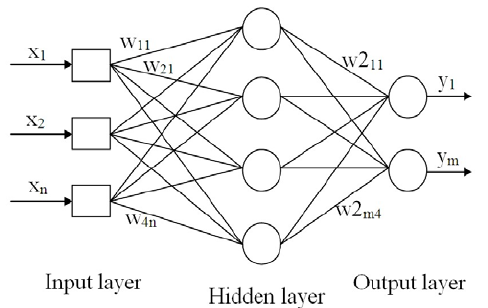
\includegraphics[width=.35\textwidth]{images/A-schematic-diagram-of-a-Multi-Layer-Perceptron-MLP-neural-network.png}
		\label{fig:mlayer-perceptron}}
	\quad\quad
	\subfigure[A single perceptron, copied from \citet{Deshpande2017}.]{
		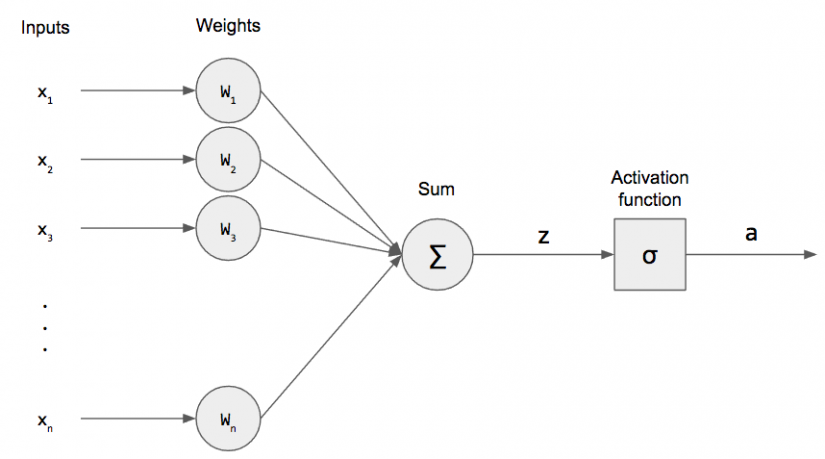
\includegraphics[width=.35\textwidth]{images/Single-Perceptron-825x459.png}
		\label{fig:single-perceptron}}
	\caption{A multilayer perceptron (a) is comprised of layers of individual perceptrons (b). TODO: reproduce myself}
	\label{fig:simple-ann}
\end{figure}
% directed acyclic graph, where nodes in the graph represent operations on data, and edges represent the flow of data through the graph. 
%This thesis will restrict itself to discussion of feedforward neural networks. 
%A feedforward neural network is an ANN where 
%Any recurrence will be unrolled to form a feedforward network. A feedforward 

\par
The set of parameters $\vtheta$ is usually learned, or trained, by stochastic gradient descent \citep{Bottou2011}.
Consider an ANN producing an approximated output $\hat{\vy} = f(\vx; \vtheta)$ and a cost function $J(\vy, \hat{\vy}) = J(\vy, \vx, \vtheta)$, with  $J$ being a differentiable function of its inputs, $\vy$ being the correct output of $f^*$, and $\vtheta$ being randomly initialized.
The cost function produces a scalar describing the error between $\vy$ and $\hat{\vy}$.
A common example of this is sum squared error, where $J(\vy, \hat{\vy}) = \sum_{n=o}^{i}(|\vy_n - \hat{\vy}_n|^2)$.
The gradient of $J$ with respect to the parameters is given by $\nabla_{\vtheta}J(\vy, \vx, \vtheta)$ and indicates the direction in which to move $\vtheta$ in order to increase $J$.
By iteratively applying $\vtheta = \vtheta - \epsilon \nabla_{\vtheta}J(\vy, \vx, \vtheta)$ (where $\epsilon$ is a scalar constant referred to as the learning rate), the value of $\vtheta$ will be modified such that $J(\vy, \vx, \vtheta)$ is minimized - thus maximizing the approximation accuracy of $f$.
$\vx$ and $\vy$ must be a randomly selected pair from the training set in order for this training process to represent the whole training dataset.
Whether this minimization lands on a global or local minimum is dependant on the function $J$.
\par


\section{Problem formation and scope}
The aim of this thesis is to build upon existing research and develop a load forecasting system which can predict future load based on weather, holiday periods, car movement, and other factors. 
Bruny Island and the NAC will be used as a case study. 
The forecasting system will be equally applicable to any power system network.
\\
Specifically, the system will have the following properties:
\begin{itemize}
	\item The system will produce a forecast up to 24 hours in the future in 15- to 60-minute intervals. This will be a rolling forecast that can be re-calculated at any time.
	\item The forecast will be able to begin from any point time.
	\item The forecast will predict load in MVA at each interval.
	\item The forecast system will be aimed at predicting aggregate load at the feeder level. That is, between approximately 0.5 and 10MVA.
	\item The forecast system will be especially tuned to predict load during holiday periods.
\end{itemize}

\chapter{Analysis and methodology}

\section{Time series forecasting - general model structure}
A model for time series forecasting must be structured in the following way.
As input, it must take a sequence of vectors, with each vector representing a single point in time, and each element of the vector representing an element of the time series.
As output, it must similarly produce a sequence of multivariate vectors.
In the case that the model is forecasting only a single time series, the output vectors will have only a single element each.
This structure is presented in Figure \ref{fig:forecast-model}.

\begin{figure}
	\centering
	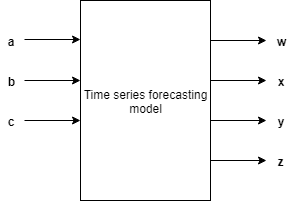
\includegraphics[width=0.35\linewidth]{images/forecast-model}
	\caption{A time series forecasting model takes a sequence of vectors, $\va, \vb, \vc$, as input and produces a sequence of vectors, $\vw, \vx, \vy, \vz$, as output. Note the number of input and output vectors is able to vary.}
	\label{fig:forecast-model}
\end{figure}

This structure is identical to that used for neural machine translation (NMT), where a source sentence/phrase is translated from one language, say English, to another language such as Dutch \citep{Cho2014}.
In NMT, a word is represented by a vector, and a sentence is represented by a sequence of vectors.

\par
This section will investigate the performance of several of the best performing NMT architectures when applied to time series forecasting.

\subsection{Investigated models}
The following NMT models will be investigated and their results in time series forecasting compared
\begin{itemize}
	\item sequence to sequence (S2S) \citep{Cho2014a} long short term memory (LSTM) \citep{hochreiter1997long}
	\item S2S LSTM with attention \citep{luong2015effective}
	\item S2S gated recurrent unit (GRU) \citep{Cho2014a} and S2S GRU with attention
	\item Transformer \citep{Vaswani2017}
\end{itemize}

Additionally, I will compare them to the following traditional methods
\begin{itemize}
	\item ARIMA and related methods
	\item support vector regression
	\item I'll probably add a few more as I further work on the state of the art section.
\end{itemize}

\subsection{Evaluation tasks}
The following time series forecasting tasks will be used to evaluate the models
\begin{itemize}
	\item forecasting a pure sine wave given its past values
	\item forecasting a sine wave with normally distributed noise given its past values
	\item forecasting a signal comprised of several sine waves with normally distributed noise given past values
	\item forecasting the Bruny Island load data - no priority given to special days.
\end{itemize}

\subsection{Evaluation Results}

\section{Transformer}
\hl{My preliminary investigations show that the transformer architecture is the best, or at least equal best but likely with less expensive training. This is consistent with \protect\cite{Song2017} and \protect\cite{Vaswani2017}}\\
\par
The transformer is a neural network architecture that is currently the state of the art in NMT \citep{Vaswani2017}.
This architecture will be discussed in detail. 

\subsection{Overview}
overview of the transformer architecture.
\begin{itemize}
	\item encoder and decoder
	\item input embedding
	\item positional encoding
	\item multi-head attention
	\item residual connections
	\item feed forward
	\item layer normalization
	\item 
\end{itemize}

\subsection{Input embedding}
convolutional embedding as per \citep{Song2017} (a paper using the transformer architecture to perform classification based on time series).

\subsection{Positional encoding}
Every input vector, $\vb_i$, has a vector added to it, $\vp_i$, depending on its position, $i$, in the input.
$\vp_i$ is trainable - it is drawn from $\vtheta$.

\subsection{multi-head attention}
I need to research this further before writing about it.

\subsection{residual connections}

\subsection{Feedforward}

\subsection{Normalization}

\subsection{etc.}

\subsection{Training}
Discuss how the decoder is used in training and inference modes.
Causality, iterative inference.
	
\chapter{Results}
This chapter presents case studies of Bruny Island and ISO New England using the proposed forecasting models.

\section{Bruny Island}
Bruny Island, shown in Figure \ref{fig:bruny_map}, is located approximately two kilometres off the coast of south-east Tasmania with a permanent resident population of approximately 800 people.
The island is a popular holiday destination, with Easter periods typically experiencing an influx of up to 500 cars in a single day.
The island is supplied by two feeders, depicted in Figure \ref{fig:bruny_network}, with  one feeder supplying a small portion of the island to the North and the other supplying the main portion of the island to the South.
This case study deals only with the feeder supplying the main portion of the island to the South.

During holiday period morning and afternoon peaks the submarine feeder reaches its capacity and a diesel generator located on the island is used to reduce the feeder load.
The substantial increase in load over the Easter holiday period for multiple years can be seen in Figure \ref{fig:bruny_easter}.

To avoid the use of the generator, the CONSORT project installed a set of residential batteries on the island for the purposes of peak-shifting.
These batteries are coordinated by the network aware coordination algorithm (NAC).
In order to peak-shift while making efficient use of the batteries, the NAC requires an accurate forecast of load with a 24-hour horizon and 30-minute resolution.

The proposed forecasting models were evaluated on historical data, with the details of the implementations and the results presented in the following sections.
A transformer-based model was implemented for online forecasting as part of the NAC, with details given in section \ref{consort-eval}.

\begin{figure}[htbp]
	\centerline{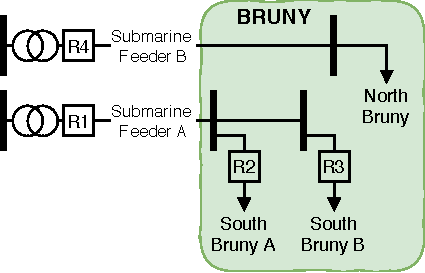
\includegraphics[width=.45\textwidth]{images/bruny_single_line.pdf}}
	\caption{Single line schematic of the distribution network on Bruny Island.}
	\label{fig:bruny_network}
\end{figure}

\begin{figure}[htbp]
	\centerline{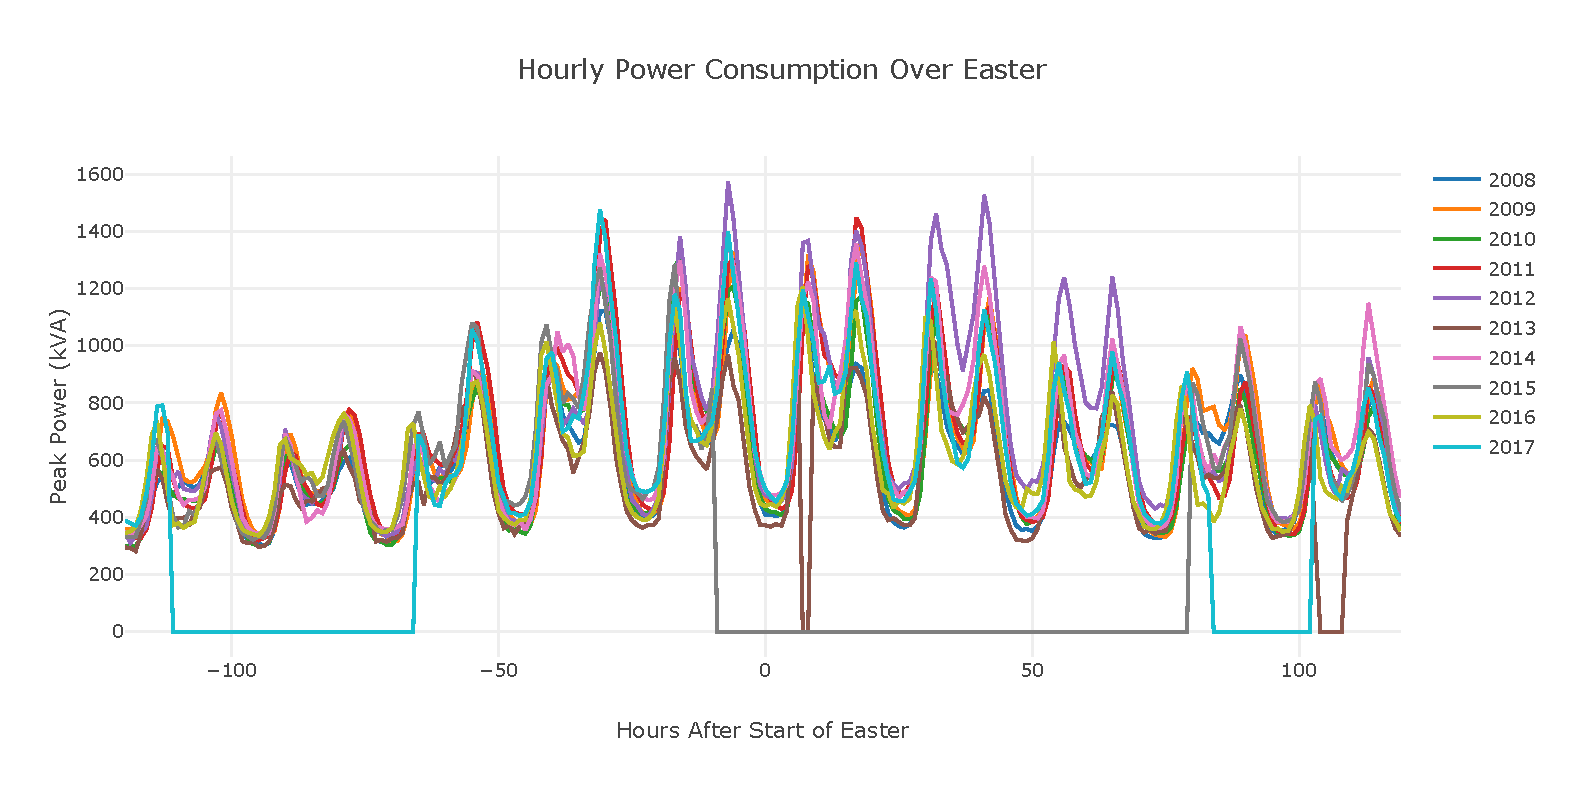
\includegraphics[width=.9\textwidth]{images/easter_bruny.pdf}}
	\caption{Easter load on Bruny Island 2008 through 2017.
		Unusable missing/bad data can also be seen in this graph.}
	\label{fig:bruny_easter}
\end{figure}

\subsection{Data analysis}
\label{bruny-data-analysis}

In section \ref{patterns-profiles} the general properties of load profiles and how they are influenced by exogenous factors was discussed. Now, these general properties will be briefly investigated for the Bruny Island feeder.
\subsubsection{Available data}
The following data is available:
\begin{itemize}
	\item Apparent power measured at recloser R1 (figure \ref{fig:bruny_network}) between January 1, 2007 and June 25, 2018
	\item Ambient Temperature, solar irradiance, humidity, and wind speed at Lenah Valley between October 1, 2009 and June 25, 2018
	\item Vehicle movement data in 10 minute resolution between June 4, 2015 and March 24, 2018
\end{itemize}	
Vehicle movement data is provided as a set of observations every 10 minutes recording the number of vehicles arriving on the island, and the number of vehicles departing the island.
By integrating this, a relative number of vehicles on the island can be established.
There is a significant amount of bad or missing data throughout these datasets which has been handled by limiting the use of data where there are too many missing or bad values.

\subsubsection{Analysis}
Figure \ref{fig:load-profiles} shows apparent power draw on Bruny Island over a winter week, a summer week, and over an entire year.
These two weeks were selected to avoid special days such as holidays and are representative of typical weeks.
Several differences can be seen between the summer and winter weeks.
In Summer, the midday load is about the same as the overnight load, whereas in Winter, it is quite different.
Summer afternoon peaks are smaller than the morning peaks, whereas in winter they are similar.
At a high level, it is clear that the load is generally larger in winter -- likely as a result of increased residential heating.
An intuitive reaction to this might be to use different forecasting models for summer and winter - but of course then a delineation must be decided on for when to switch between the two models.
As one of the aims of the forecasting system is to be practical to implement, it is desirable to have a single system that is be able to forecast both summer and winter.
By supplying temperature as an exogenous input this should be possible.

\begin{figure}[htbp]
	\centering
	\subfigure[Load over a single summer week in 2018.]{
		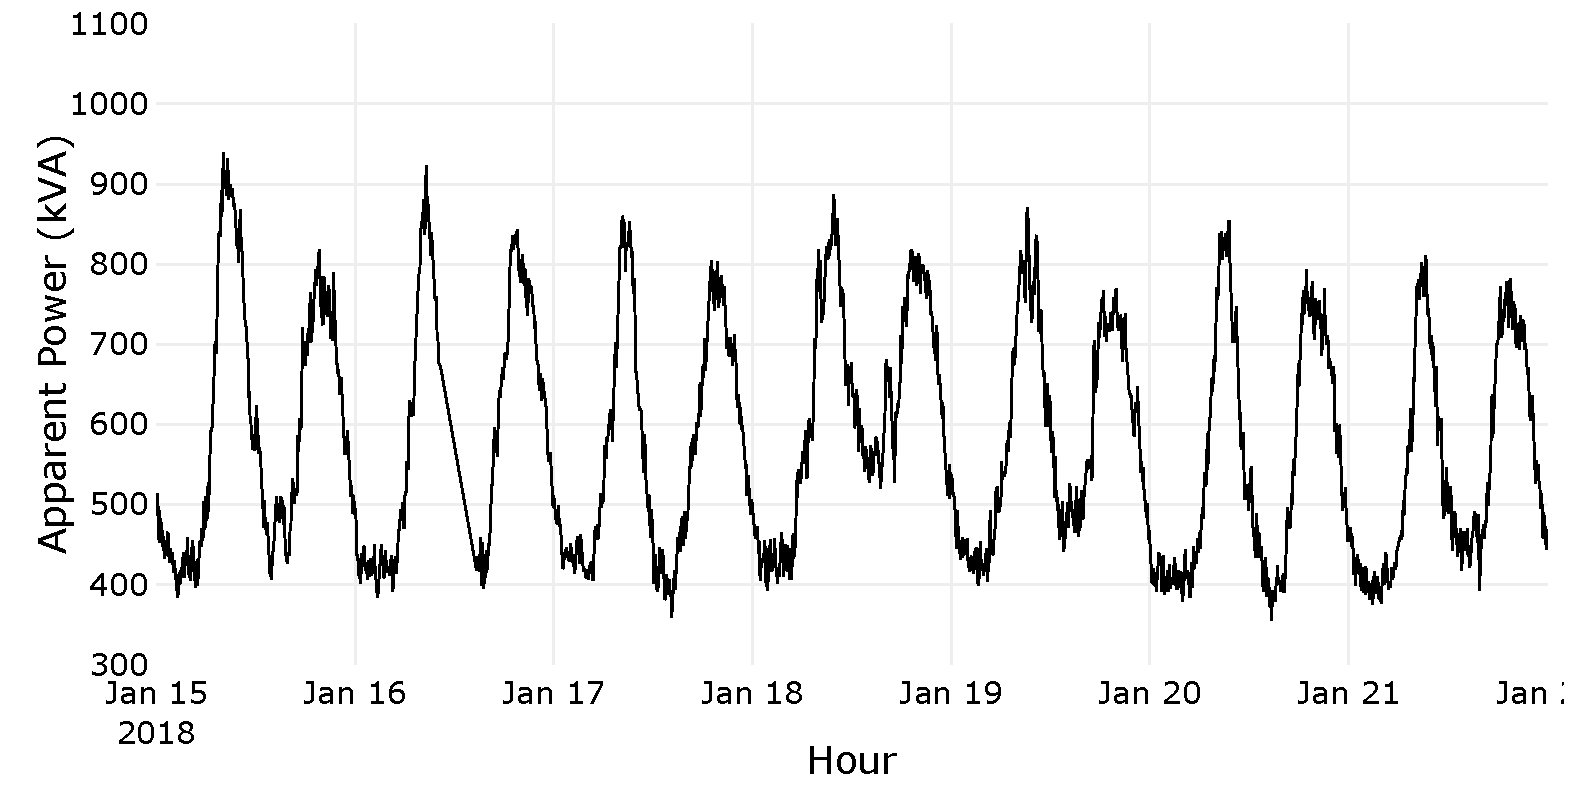
\includegraphics[width=0.8\textwidth]{images/simple-week-summer.pdf}
		\label{fig:simple-week-summer}}
	\vfil
	\subfigure[Load over a single winter week in 2017.]{
		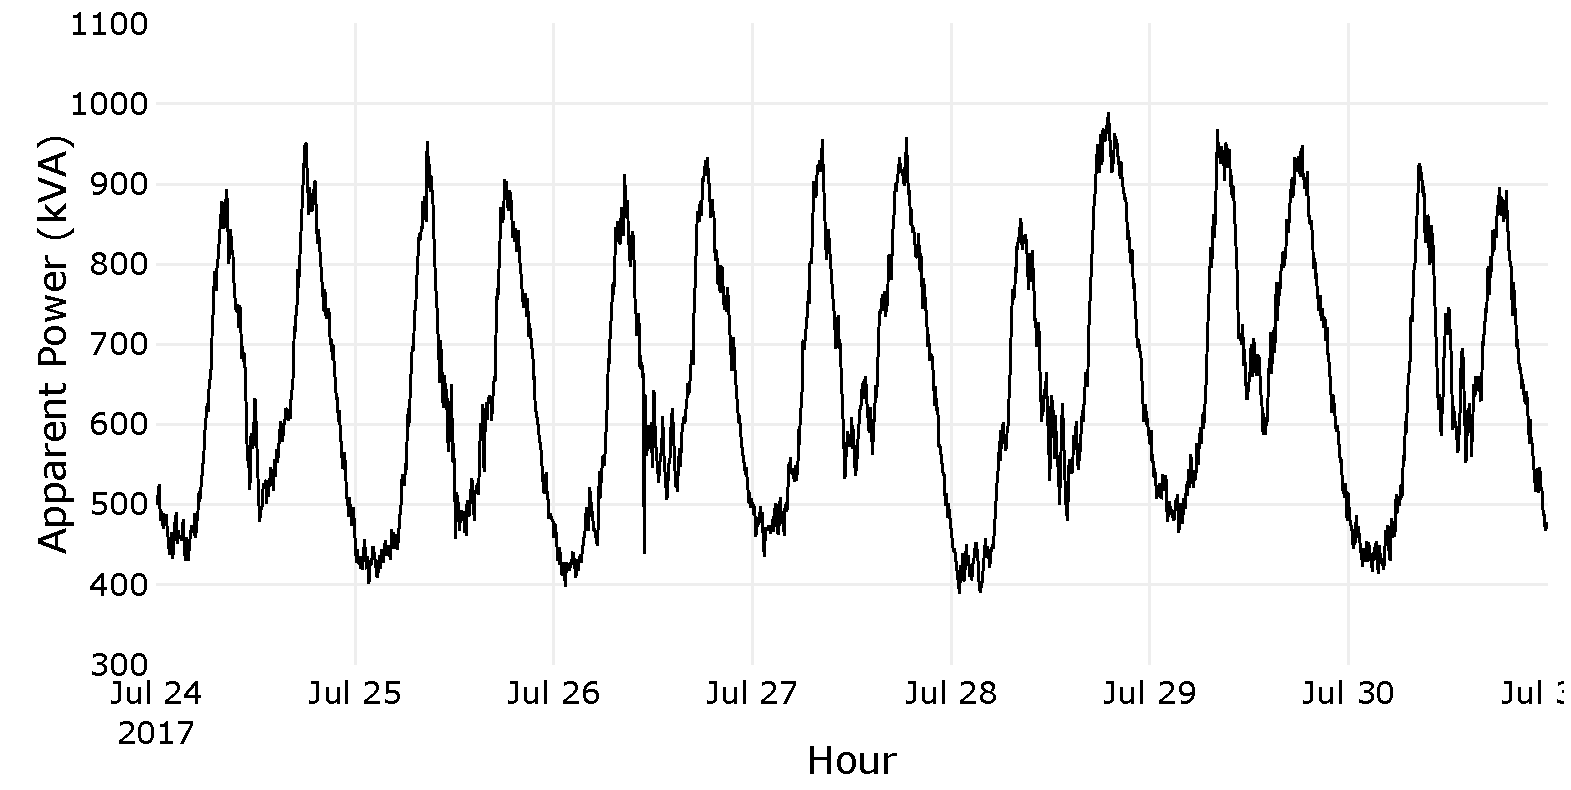
\includegraphics[width=0.8\textwidth]{images/simple-week-winter.pdf}
		\label{fig:simple-week-winter}}
	\vfil
	\subfigure[Peak daily load and peak daily temperature over all of 2017.]{
		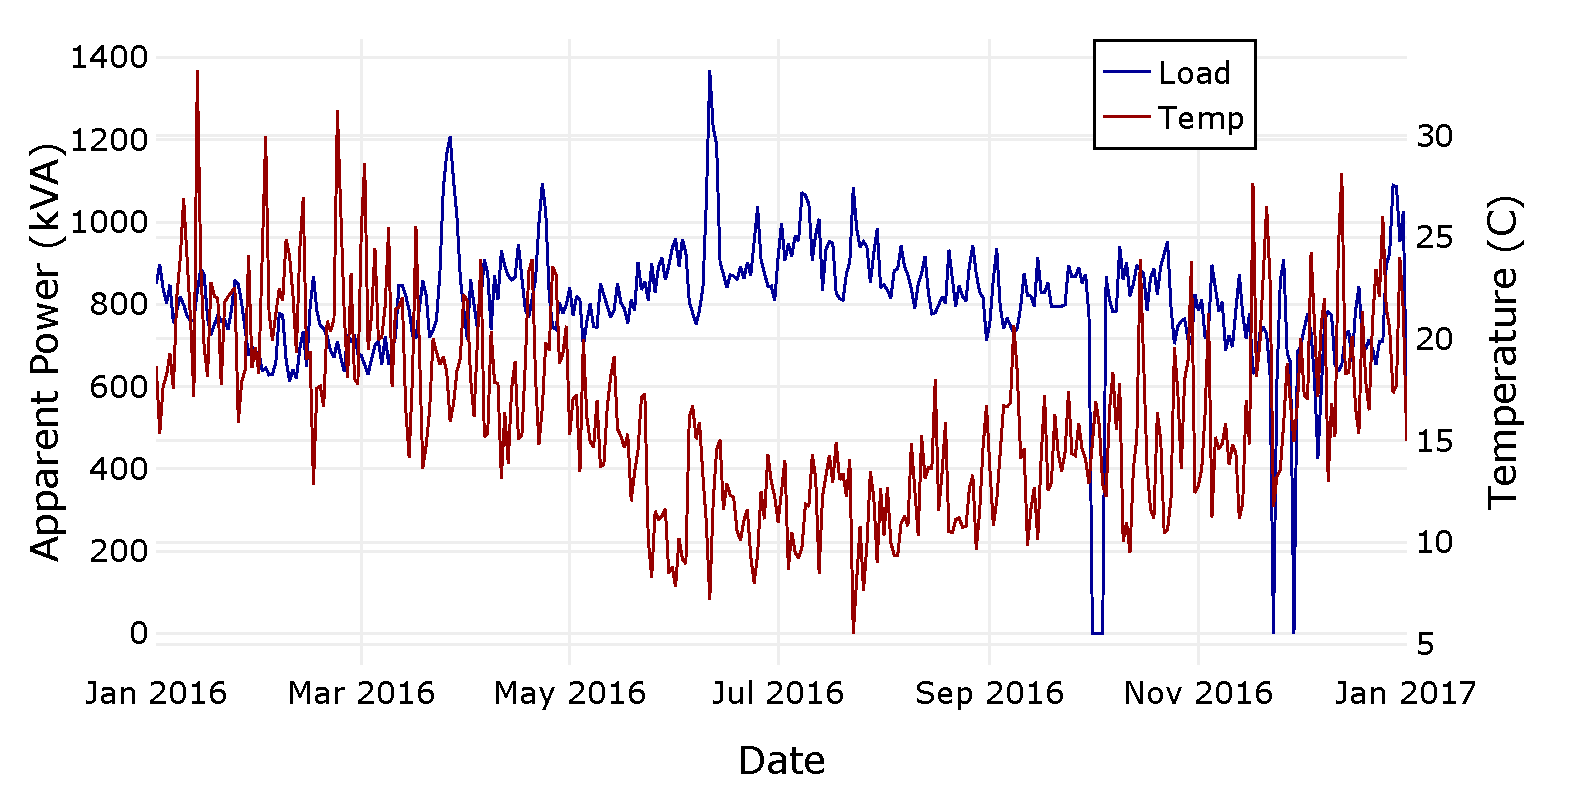
\includegraphics[width=0.8\textwidth]{images/max-load-max-temp.pdf}
		\label{fig:max-load-max-temp}}
	\caption{Bruny Island load profiles.}
	\label{fig:load-profiles}
\end{figure}

It was mentioned in section \ref{patterns-profiles} that weekends and weekdays tend to have different load profiles, but this is not immediately obvious from figure \ref{fig:load-profiles}.
Figure \ref{fig:average-profiles} shows this difference between days of the week.
What is immediately obviously is that the differences between days of the week are not restricted to 24 hour bounds - the different load profile shapes gently merge into each other over the course of an afternoon or morning.
% This is an especially important observation for a forecasting system that needs to be able to perform forecasts not just at a single time each day, but at any time.
It can be seen that the Friday profile morphs into the Saturday profile during the afternoon, perhaps as people arrive on the island for the weekend, and the Sunday profile morphs into a weekday profile over the afternoon, perhaps as people depart the island.

Figures \ref{fig:average-arriving} and \ref{fig:average-departing} further support that the changes in load profiles are a result of people arriving on or leaving the island.
It can be seen that many vehicles tend to arrive on the island on Friday afternoon, leading to the change in load profile between Friday and Saturday.
Likewise, many vehicles leave the island on Sunday afternoon, shifting the load profile from Sunday to a weekday.

This brief investigation serves to highlight some of the challenges that the load forecasting system must handle.

\begin{figure}[htbp]
	\centering
	\subfigure[Average load profiles for each day of the week.]{
		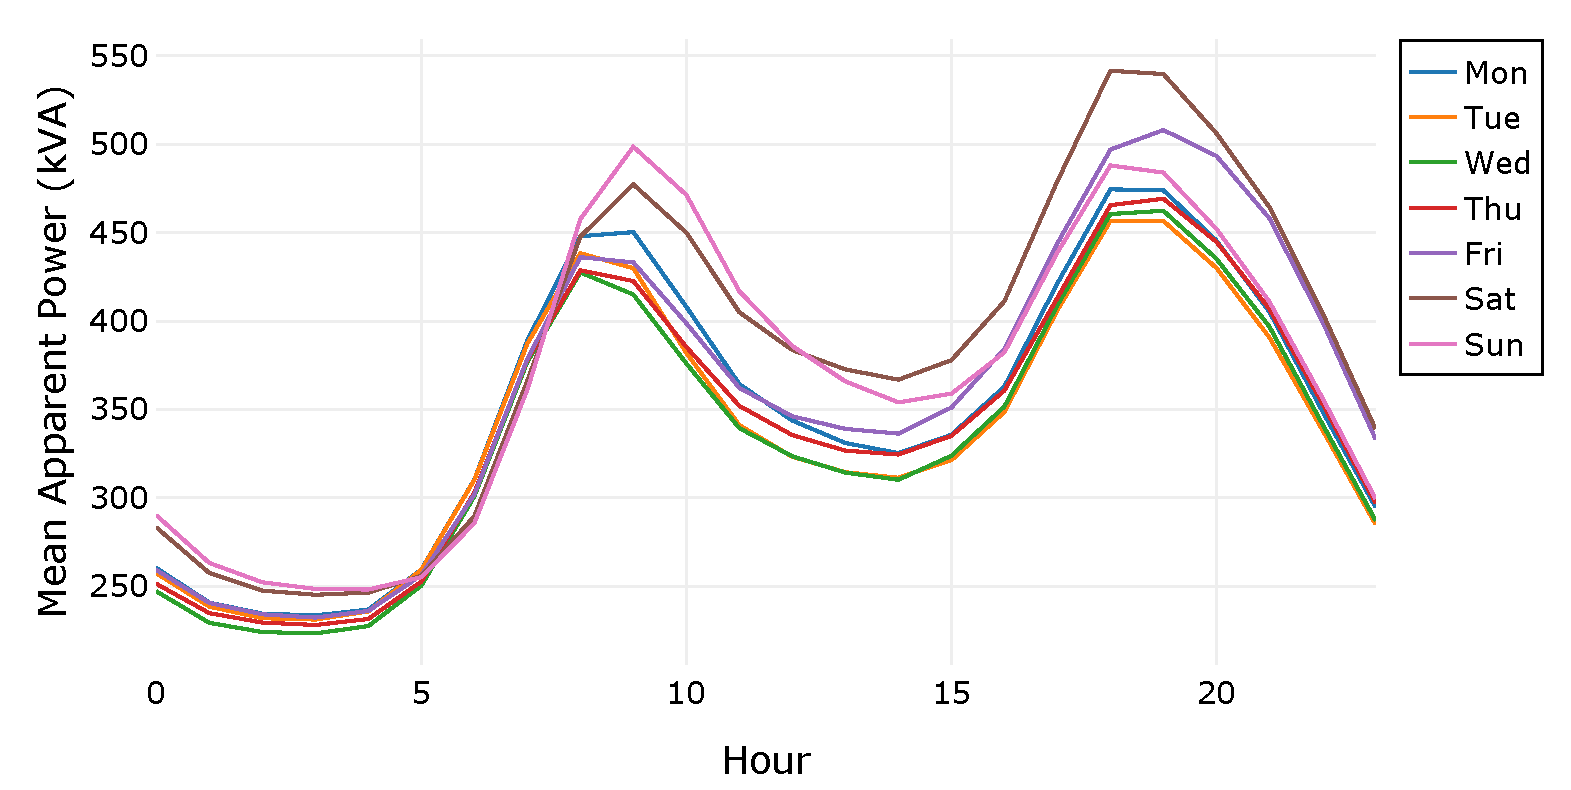
\includegraphics[width=.8\textwidth]{images/average-profiles.pdf}
		\label{fig:average-profiles}}
	\vfil
	\subfigure[Average number of cars arriving on the island for each day of the week.]{
		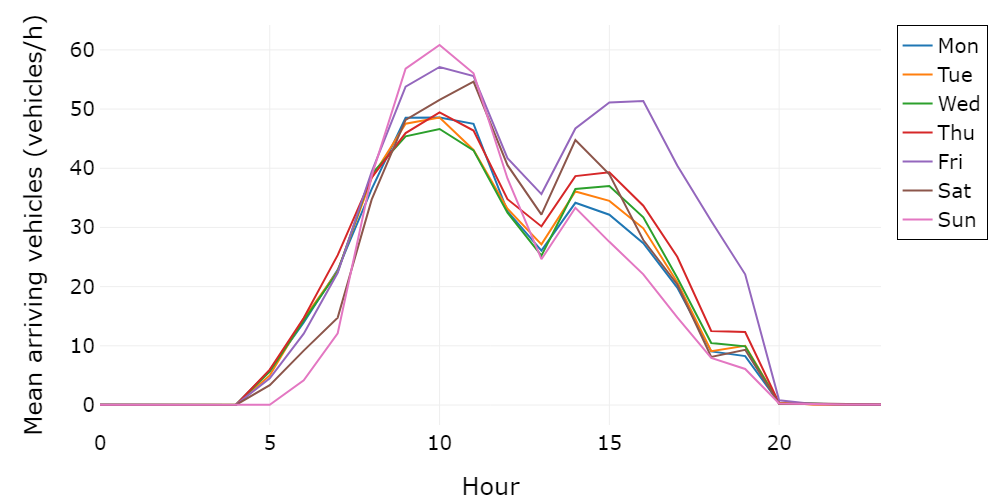
\includegraphics[width=.8\textwidth]{images/average-arriving}
		\label{fig:average-arriving}}
	\vfil
	\subfigure[Average number of cars leaving the island for each day of the week.]{
		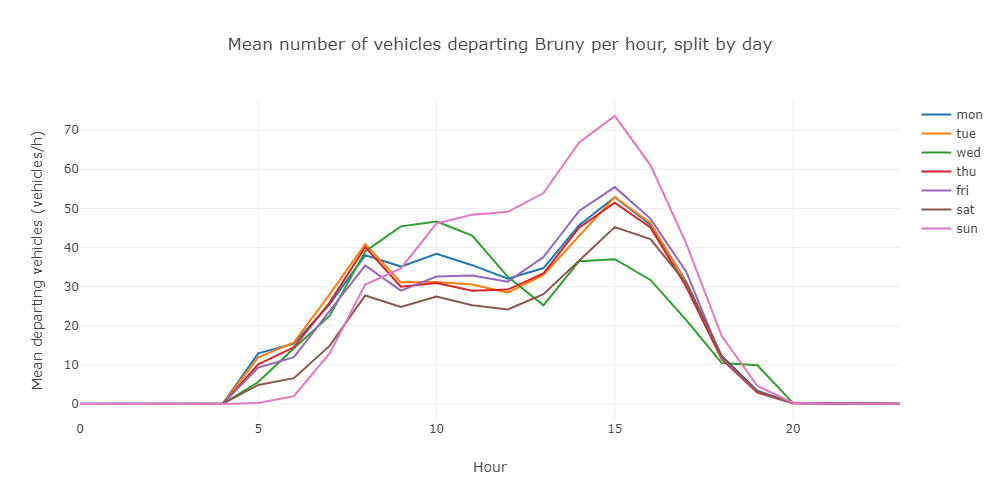
\includegraphics[width=.8\textwidth]{images/average-departing}
		\label{fig:average-departing}}
	\caption{Bruny Island average load profiles.}
	\label{fig:average-load-profiles}
\end{figure}

\subsection{Forecasting tasks}
\label{forecasting-tasks}
The forecasters were evaluated on several tasks, shown in table \ref{table:offline-results-bruny-lscape}, and discussed in section \ref{bruny_offline_results}.
The hourly task has the forecaster predict the future 24 hours of load in one-hour resolution given the previous 24 hours of load and the future 24 hours of date/time, holiday, and temperature data.
The half-hourly task is the same as hourly, except using half-hour resolution data.
The hourly long task has the forecaster predict the future 24 hours of load in one-hour resolution given the previous 168 hours (one week) of load and the future 24 hours of date/time, holiday, and temperature data.
The hourly ($c$=3) task is the same as the hourly task but with the loss function modified, as described in section \ref{train-reg}, with $c=3$.

The tasks listed as being ``with similar profiles" include five similar profiles ($k=5$, as described in the following section \nameref{data-model-config}).
The tasks that do not list similar profiles have no similar profiles, $k=0$.

\subsection{Data and  model configuration}
\label{data-model-config}
The available data was split into a training set (October 1 2009 through February 15 2014) and a testing set (February 16 2014 through June 25 2018).
For the hourly task, the network was supplied with data in hourly resolution from the previous and future 24 hours:
\begin{itemize}
	\item The previous 24 hours of load, $\vl = [ l_1 \: l_2 \: ...  \: l_{24}]^\top$, with $l_{24}$ being the most recent load.
	\item Temperature for the future 24 hours, $\vt = [t_1 \: t_2 \: ... \: t_{24}]^\top$, with $t_1$ being the soonest point in the future.
	\item Day of the week as an integer from 0 to 6 (local time) over the future 24 hours, $\vd = [d_1 \: d_2 \: ... \: d_{24}]^\top$, with $d_1$ being the soonest point in the future.
	\item Minutes since midnight (local time) for the future 24 hours, $\vm = [m_1 \: m_2 \: ... \: m_{24}]^\top$, with $m_1$ being the soonest point in the future.
	\item Boolean 1 or 0 indicating whether it is a holiday at each hour over the next 24 hours, $\vh = [h_1 \: h_2 \: ... \: h_{24}]^\top$, with $h_1$ being the soonest point in the future.
	\item Holiday type as an integer from 0 to $n$ at each hour over the future 24 hours, where there are $n$ different holidays in the year, $\vg = [g_1 \: g_2 \: ... \: g_{24}]^\top$, with $g_1$ being the soonest point in the future.
	\item Month of the year from 0 to 11 (local time) over the future 24 hours, $\vn = [n_1 \: n_2 \: ... \: n_{24}]^\top$, with $n_1$ being the soonest point in the future.
\end{itemize}

Additionally, similar profile data was constructed for $k$ similar days, as described in section \ref{simperiod}.
The weights used are given in table \ref{table:offline-parameters}.
The extremely large weights are used to ensure that similar profiles are always selected from the same month and day of month/day of week unless there are none available.
The similar day data is aligned with the same points in time as the $\vt$ vector.
The order in which the similar days were added to the $\mX$ input matrix was randomized during both training and testing/inference.
The similar profile data is:

\begin{itemize}
	\item 24 hours of similar profile load $\vl_{sk} = [ l_{sk1} \: l_{sk2} \: ... \: l_{sk24}]^\top$.
	\item 24 hours of similar profile temperature (corresponding to the same points in time as $\vl_{sk}$), $\vt_{sk} = [ t_{sk1} \: t_{sk2} \: ...  \: t_{sk24}]^\top$.
\end{itemize}

This data was concatenated to form the input matrix given in equation \ref{eq:input-matrix}.

\begin{equation} \label{eq:input-matrix}
\mX = [ \vl \: \vt \: \vd \: \vm \: \vh \: \vg \: \vn \: \vl_{s1} \: \vt_{s1} \: \ldots \: \vl_{sk} \: \vt_{sk}] \in \mathbb{R}^{24 \times (7 + 2k)}
\end{equation}

The half-hourly configuration is the same as the hourly configuration, except all vectors contain 48 elements (representing 24 hours of data) and so $\mX \in \mathbb{R}^{48 \times (7 + 2k)}$.

The hourly long configuration modifies only the $\vl$ vector, such that $\vl = [ l_1 \: l_2 \: ...  \: l_{168}]^\top$ representing one week of hour-resolution data, with $l_{168}$ being the most recent observation.
The other vectors were zero padded to match this length.
With $\vz \in \mathbb{R}^{144}$ being a zero vector, and $\hat{\vv} = [\vz^\top \vv^\top]^\top$ for any vector $\vv$, the input $\mX$ is given by equation \ref{hourly-long-x}.
\begin{equation}
\label{hourly-long-x}
\mX = [ \hat{\vl} \: \hat{\vt} \: \hat{\vd} \: \hat{\vm} \: \hat{\vh} \: \hat{\vg} \: \hat{\vn} \: \hat{\vl_{s1}} \: \hat{\vt_{s1}} \: \ldots \: \hat{\vl_{sk}} \: \hat{\vt_{sk}}] \in \mathbb{R}^{168 \times (7 + 2k)}
\end{equation}

The forecasting models were configured with the parameters given in table \ref{table:offline-parameters} and trained for $10^5$ iterations.
All the models presented in section \ref{ana-meth} are evaluated.
The ``Transformer" model is the transformer with teacher forcing enabled, and the ``Transformer no TF" model is the transformer with teacher forcing disabled.

\begin{table}[htbp]
	\caption{Offline Evaluation model parameters.}
	\begin{center}
	\begin{tabular}{lclc}
	\multicolumn{1}{c}{\textbf{Model/Method}} & \textbf{Parameter} & \textbf{Description}                 & \textbf{Value} \\ \cline{1-4} 
	
	\multirow{6}{*}{\shortstack[l]{SARIMAX}}       
	& $p$                & AR model order     					& 2              \\
	& $d$                & Number of differences   		        & 1             \\
	& $q$                & MA model order           			& 1              \\
	& $P$                & Seasonal AR model order              & 1            \\
	& $D$                & Number of seasonal differences       & 1              \\
	& $Q$                & Seasonal MA model order              & 1             \\
	& $s$                & Period of seasonality		        & 24             \\ \cline{1-4} 
	
	\multirow{6}{*}{\shortstack[l]{Sequence to\\Sequence}}       
	& $L$                & Number of encoder and decoder layers & 2              \\
	& $d$                & Hidden dimension                     & 16             \\
	& $D$                & Dropout fraction                     & 0            \\
	& $c$                & Loss function modifier               & 0              \\
	& $l$                & Learning rate 			            & 0.001             \\
	& -                  & Training batch size                  & 16             \\ \cline{1-4} 
	
	\multirow{6}{*}{\shortstack[l]{Transformer}}       
	& $L$                & Number of encoder and decoder layers & 2              \\
	& $d$                & Hidden dimension                     & 16             \\
	& $h$                & Number of attention heads            & 2              \\
	& $D$                & Dropout fraction                     & 0.2            \\
	& $c$                & Loss function modifier               & 0              \\
	& $l$                & Learning rate 			            & 0.001              \\
	& -                  & Training batch size                  & 16             \\ \cline{1-4} 
	
	\multirow{6}{*}{\shortstack[l]{Universal Transformer}}      
	& $L$                & Number of encoder and decoder layers & 2              \\
	& $d$                & Hidden dimension                     & 16             \\
	& $h$                & Number of attention heads            & 2              \\
	& $D$                & Dropout fraction                     & 0.2            \\
	& $c$                & Loss function modifier               & 0              \\
	& $l$                & Learning rate 			            & 0.001              \\
	& -                  & Training batch size                  & 16             \\ \cline{1-4} 
	
	\multirow{6}{*}{\shortstack[l]{Similar\\Profile\\Selection}}
	& -                  & Maximum future temperature weight    & 10             \\
	& -                  & Minimum future temperature weight    & 20             \\
	& -                  & Maximum past load weight             & 30             \\
	& -                  & Holiday type weight                  & 1e9            \\
	& -                  & Day of week weight                   & 1e6            \\
	& -                  & Day of month weight                  & 1e6            \\
	& -                  & Month of year weight                 & 1e6           
\end{tabular}
		\label{table:offline-parameters}
	\end{center}
\end{table}


\subsection{Offline evaluation results}
\label{bruny_offline_results}
The forecaster was trained on the training dataset (October 1 2009 through February 15 2014) and tested on the testing dataset (February 16 2014 through June 25 2018).
The train and test datasets were then switched in order to cross-validate the results.
All presented results are the average of the cross validated results.
Results are shown in table \ref{table:offline-results-bruny-lscape}.

Both the mean absolute percentage error (MAPE) and mean absolute error (MAE) are shown.
These metrics are calculated for all load, for load only over 1MVA, and for load that is at a first large peak.
A first large peak is a morning or afternoon peak that is over 1MVA and is greater than 36 hours after any previous peak that was over 1MVA.
The first large peak metric is used because it is generally considered difficult to forecast.
These two metrics allow the performance of the system on anomalous holiday periods to be more directly evaluated.

The SARIMAX model proved to produce results that are relatively poor compared to the other models, and so was not considered beyond the hourly without similar days task.
The universal transformer is consistently a poor performer, never producing the best results for any task or metric.
The transformer model is generally outperformed by, or at least very similar to, the transformer without teacher forcing model.
Excluding these models, it is clear that there is no model which is overall superior between the S2S and transformer without teacher forcing models.

The S2S model appears to excel at the hourly task, achieving the best MAPE scores above 1 MVA and at first large peak, while also being close to the transformer without teacher forcing on the overall MAPE score.
The S2S model generally produces good results across the board.

The transformer without teacher forcing is generally good at minimizing the overall MAPE score.
It also performs exceedingly well in the hourly long task, achieving the lowest overall MAPE while the other two metrics are close to the hourly with similar and $c=3$ task.
This model is also arguably the best at the half-hourly tasks, achieving the best results on the majority of metrics across both tasks.
The dominance of the transformer-based models on the half-hourly and hourly long tasks is likely a result of the transformer's ability to handle long sequence lengths,
as discussed in section \ref{sec:transformer}.

The hourly with $c=3$ tasks show no consensus on which model is generally superior.
Interestingly, the hourly long task achieves similar results to the hourly with $c=3$ with similar profiles task.

\afterpage{%
	\clearpage% Flush earlier floats (otherwise order might not be correct)
	\thispagestyle{empty}% empty page style (?)
	\begin{landscape}% Landscape page
		\centering % Center table
		\begin{table}[htbp]
			\caption{Offline evaluation results.}
			% \begin{center}
				\begin{tabular}{llcccccc}
					\multicolumn{1}{c}{\textbf{Task}} &
					\multicolumn{1}{c}{\textbf{Model}} & 
					\multicolumn{1}{c}{\textbf{\shortstack[c]{MAPE\\(\%)}}} &
					\multicolumn{1}{c}{\textbf{\shortstack[c]{MAE\\(kVA)}}} & 
					\multicolumn{1}{c}{\textbf{\shortstack[c]{MAPE over\\1 MVA (\%)}}} &
					\multicolumn{1}{c}{\textbf{\shortstack[c]{MAE over\\1 MVA (kVA)}}} &
					\multicolumn{1}{c}{\textbf{\shortstack[c]{MAPE at first\\large peak (\%)}}} &
					\multicolumn{1}{c}{\textbf{\shortstack[c]{MAE at first\\large peak (kVA)}}} \\ \cline{1-8}
					
					\multirow{4}{*}{\shortstack[l]{Hourly}}       
					& SARIMAX           &         14.34  &         82.1  &         12.31  &         137.7  &         18.86  &         200.9 	\\ % (2,1,1)(1,1,1,24)/_cv
					& S2S      			&          7.85  &         42.8  &  \textbf{9.87} & \textbf{110.6} & \textbf{11.42} & \textbf{112.6}	\\ % 
					& Transformer       &          7.82  &         43.1  &         10.33  &         115.1  &         13.00  &         140.1 	\\ % 
					& Transformer no TF &  \textbf{7.77} & \textbf{42.6} &         11.45  &         128.9  &         13.24  &         142.0 	\\ % 130 131
					& U. Transformer    &          8.20	 &         46.0  &         11.72  &         131.6  &         14.52  &         155.2 	\\ % 
					\cline{1-8}					
					
					\multirow{3}{*}{\shortstack[l]{Hourly\\with similar\\profiles}} 
					& S2S      			&          7.68  &         41.6  &  \textbf{9.77} & \textbf{109.6} & \textbf{11.05} & \textbf{118.7}	\\ % 
					& Transformer       &          7.40  &         40.7  &         10.25  &         115.2  &         12.45  &         133.6 	\\ % 
					& Transformer no TF &  \textbf{7.24} & \textbf{39.6} &         10.32  &         115.8  &         12.47  &         133.7    	\\ % 122 123
					& U. Transformer    &          8.15  &         44.8  &         11.10  &         123.5  &         12.67  &         135.5 	\\ % 
					\cline{1-8}					
					
					\multirow{3}{*}{\shortstack[l]{Half-\\hourly}}       
					& S2S      			&  \textbf{7.80} & \textbf{42.7} &          9.88  &         111.3  &         12.30  &         131.5 	\\ % 
					& Transformer       &          9.14  &         50.9  &         13.03  &         148.0  &         15.80  &         170.0 	\\ % 
					& Transformer no TF &          8.24  &         44.0  &  \textbf{9.03} & \textbf{101.5} & \textbf{10.22} & \textbf{110.4}  	\\ % 126 127
					& U. Transformer    &          8.60  &         48.0  &         13.60  &         154.6  &         14.33  &         154.5 	\\ % 
					\cline{1-8}					
					
					\multirow{3}{*}{\shortstack[l]{Half-hourly\\with similar\\profiles}}       
					& S2S      			&          8.44  &         45.0  &         10.23  &         116.2  &         11.10  &         119.1 	\\ % 
					& Transformer       &          7.82  &         42.5  &         10.78  &         121.6  & \textbf{10.98} & \textbf{118.5}	\\ % 
					& Transformer no TF &  \textbf{7.41} & \textbf{41.0} & \textbf{10.16} & \textbf{114.1} &         12.54  &         134.8  	\\ % 128 129
					& U. Transformer    &          9.05  &         48.1  &         10.22  &         114.6  &         11.90  &         136.0 	\\ % 
					\cline{1-8}					
					
					\multirow{3}{*}{\shortstack[l]{Hourly long\\with similar\\profiles}}       
					& S2S      			&          7.49  &         40.9  &  \textbf{9.43} & \textbf{106.2} &         10.10  &         109.5 	\\ % 
					& Transformer       &          6.97  &         38.0  &         10.82  &         122.5  &         11.30  &         121.8 	\\ % 
					& Transformer no TF &  \textbf{6.68} & \textbf{36.8} &          9.85  &         111.8  &  \textbf{9.54} & \textbf{103.1} 	\\ % 132 133
					& U. Transformer    &          6.74  &         38.5  &         10.35  &         116.1  &         12.82  &         138.2 	\\ % 
					\cline{1-8}					
					
					\multirow{3}{*}{\shortstack[l]{Hourly; $c=3$}}       
					& S2S      			&          8.96  &         46.8  &  \textbf{8.61} &  \textbf{95.9} &  \textbf{9.61} & \textbf{103.0}	\\ % 
					& Transformer       &  \textbf{8.14} & \textbf{44.5} &         10.46  &         117.5  &         12.25  &         130.9 	\\ % 
					& Transformer no TF &          8.65  &         45.4  &          9.36 &          105.0  &         10.76  &         115.1  	\\ % 134 135
					& U. Transformer    &          9.29  &         48.5  &         11.05  &         124.5  &         12.97  &         138.9 	\\ % 
					\cline{1-8}					
					
					\multirow{3}{*}{\shortstack[l]{Hourly\\with similar\\profiles; $c=3$}}       
					& S2S      			&  \textbf{8.32} & \textbf{43.8} &          9.20  &         103.1  &         10.68  &         114.8 	\\ % 
					& Transformer       &          8.58  &         45.5  &  \textbf{8.90} &  \textbf{99.5} &  \textbf{9.29} &  \textbf{99.9}	\\ % 
					& Transformer no TF &          8.86  &         45.4  &          8.99  &         101.1  &         10.21  &         109.7  	\\ % 136 137
					& U. Transformer    &          9.00  &         48.3  &         10.07  &         112.5  &          9.34  &         100.5 	\\ % 
					\cline{1-8} 
				\end{tabular}
				\label{table:offline-results-bruny-lscape}
			% \end{center}
		\end{table}
	\end{landscape}
	\clearpage% Flush page
}


\begin{figure}[htbp]
	\centerline{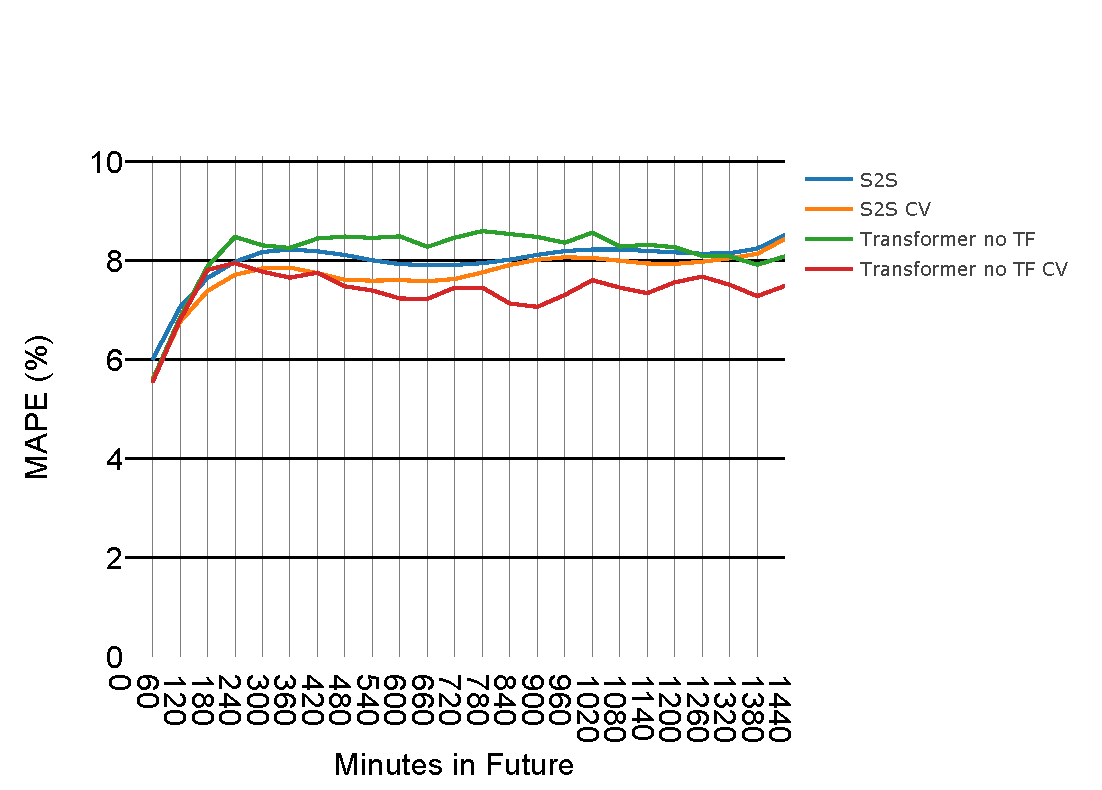
\includegraphics[width=.9\textwidth]{images/bruny_mape.pdf}}
	\caption{Mean absolute percentage error of each point in the forecasts for Bruny Island, task ``Hourly".}.
	\label{fig:bruny_mape}
\end{figure}

\begin{figure}[htbp]
	\centerline{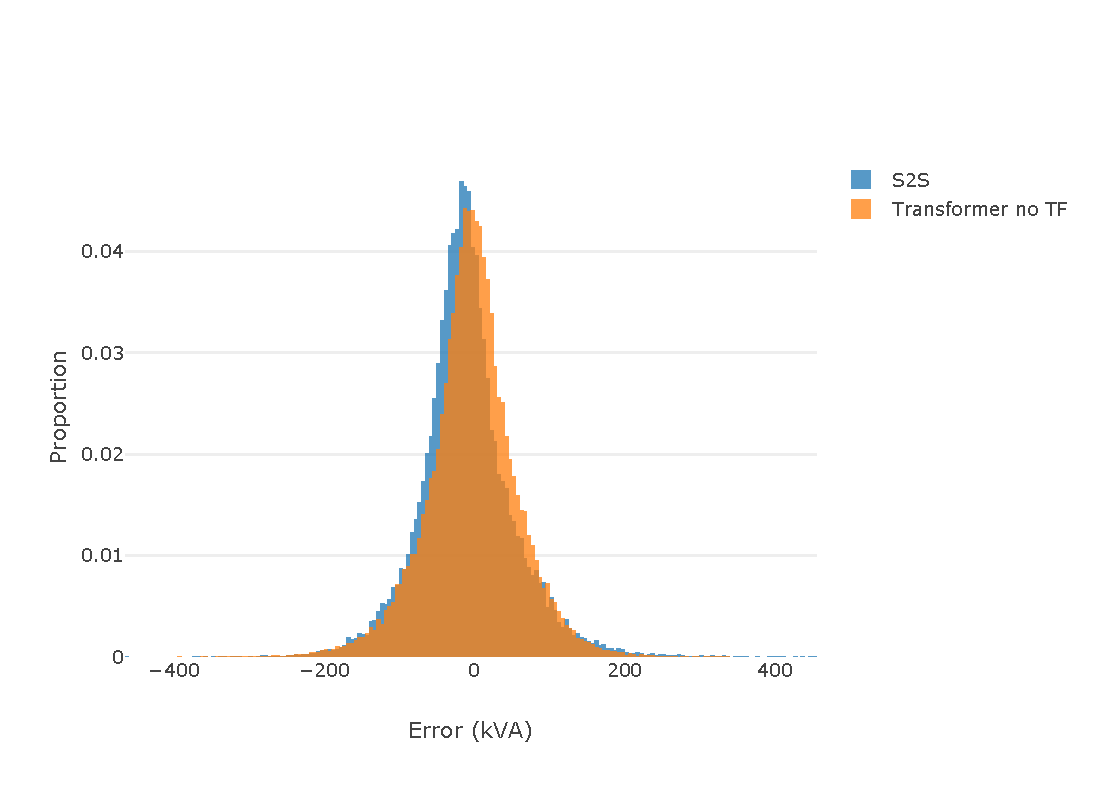
\includegraphics[width=.9\textwidth]{images/bruny_hist.pdf}}
	\caption{Distribution of forecast error corresponding to Figure \ref{fig:bruny_mape}.}
	\label{fig:bruny_hist}
\end{figure}


\subsection{Training data requirements}
Neural networks generally require large amounts of training data in order to fit the model parameters.

\subsection{Autoregression requirements}
All models presented have been supplied with at least the past 24 hour of load.
If this data is not supplied, the models are still able to forecast load.



\subsection{Online CONSORT implementation}
\label{consort-eval}
In July 2018 the load forecasting system was implemented as part of the CONSORT project and was used to assist with dispatch of residential batteries.
The model implemented was a transformer (with teacher forcing enabled), and is somewhat different to the models discussed in the offline evaluation.
Although the implemented model achieved sufficient accuracy while in use, it has since been determined to be a sub-optimal configuration.
The data and model configuration is somewhat different than described for the offline evaluation in section \ref{data-model-config}, and so this section is largely repeated here.

\subsubsection{Data and  Model Configuration}
The following data was available from 2009-2018:
\begin{itemize}
	\item Apparent power at reclosers R1 through R4 (Figure \ref{fig:bruny_network}).
	\item Temperature at Lenah Valley, Tasmania (50km from Bruny Island). 
	\item Apparent power consumption at St Helens, Tasmania.
\end{itemize}

This data was averaged to 30 minute resolution and split into a training set containing data from October 2009 through September 2014, and a testing set containing data from October 2014 through April 2018.

The network was supplied with data from the previous and future 24 hours, for a total input sequence length of 96 (representing 48 hours at 30 minute resolution).
The output sequence length was 48 (24 hours).
The data was configured differently than described in section \ref{data-model-config}.
The $\mX$ input matrix was constructed with all vectors containing 96 elements, representing the previous 24 and the future 24 hours.
The past load vector $\vl = [ l_1 \: l_2 \: ...  \: l_{48} \: 0 \: ... \: 0]^\top \in \mathbb{R}^{96}$ was populated with the past 48 load observations (representing 24 hours) and zero padded to match the shape of the rest of the data.

The following time series were supplied to the model input:
\begin{itemize}
	\item Apparent power from recloser R1 (Figure \ref{fig:bruny_network}), with future values set to zero.
	\item Temperature.
	\item Day of the week as an integer from 0 to 6 (local time).
	\item Minutes since midnight (local time).
	\item Boolean 1 or 0 indicating whether it is a holiday.
	\item Holiday type.
\end{itemize}

When used for inference, temperature forecasts were obtained from the Bureau of Meteorology.
Additionally, five similar periods were identified using data from R1 by the process described in section \ref{simperiod}.
The data over the similar periods for each of the following time series was provided as input:
\begin{itemize}
	\item Reclosers R1, R2, R3, and R4 (Figure \ref{fig:bruny_network}) (as separate time series).
	\item St Helens recloser.
	\item Lenah Valley temperature.
\end{itemize}

In total, 36 time series were provided as input to the model.
St Helens was included because it was observed to display similar patterns to Bruny Island around holiday periods.

The forecasting system was configured with the parameters in table \ref{table:parameters}, with the upper section giving transformer model parameters and the lower section giving weights used for similar period selection.
The model was trained for $10^5$ iterations.

\begin{table}[htbp]
	\caption{Case study model parameters.}
	\begin{center}
		\begin{tabular}{clc}
			%			3.\hline
			\textbf{Parameter}&\textbf{Description}&\textbf{Value} \\
			\hline
			$L$ & Number of encoder and decoder layers & 4 \\
			$d$ & Hidden dimension & 32 \\
			$h$ & Number of attention heads & 4 \\
			$D$ & Dropout fraction & 0.2 \\
			$c$ & Loss function modifier & 3 \\
			-   & Training batch size & 16 \\
			\hline
			-   & Maximum future temperature weight & 10 \\
			-   & Minimum future temperature weight & 20 \\
			-   & Maximum past load weight & 30 \\
			-   & Holiday type weight & 1e9 \\
			-   & Day of week weight & 1e6 \\
			-   & Day of month weight & 1e6 \\
			-   & Month of year weight & 1e6 \\
			
		\end{tabular}
		\label{table:parameters}
	\end{center}
\end{table}

\subsubsection{Online Evaluation}
When implemented live on the Bruny Island distribution network during the July 2018 school holiday period, as part of the CONSORT project, the forecaster was observed to reliably forecast large demand peaks.
This enabled the fleet of distributed batteries to be used effectively in providing network support via net demand peak reduction. An accurate forecast, issued early enough in advance of the occurence of the demand peak, was observed to give the batteries adequate time to store energy in the lead up to, and discharge during the demand peak period. In at least one instance over the test period this was sufficient to avoid the island's diesel generator from being used at all, when it otherwise almost certainly would have been required.
Data collected during this peak demand period can be seen in Figure \ref{fig:bruny_nac}.
The upper section shows 24 hours of historical load in black, plus the most recent 24-hour horizon forecast in dashed black (recalculated every five minutes) and all old forecasts in grey.
The lower section shows the battery charge rate, where a negative value of battery charge rate indicates the batteries are supporting the grid.

Typically the generator is switched on when load exceeds 1050 kVA.
During the first peak the graph shows the batteries supplying between 50 and 100 kW to the island.
Without this support from the batteries, the generator would have likely been required to operate.

\begin{figure}[htbp]
	\centerline{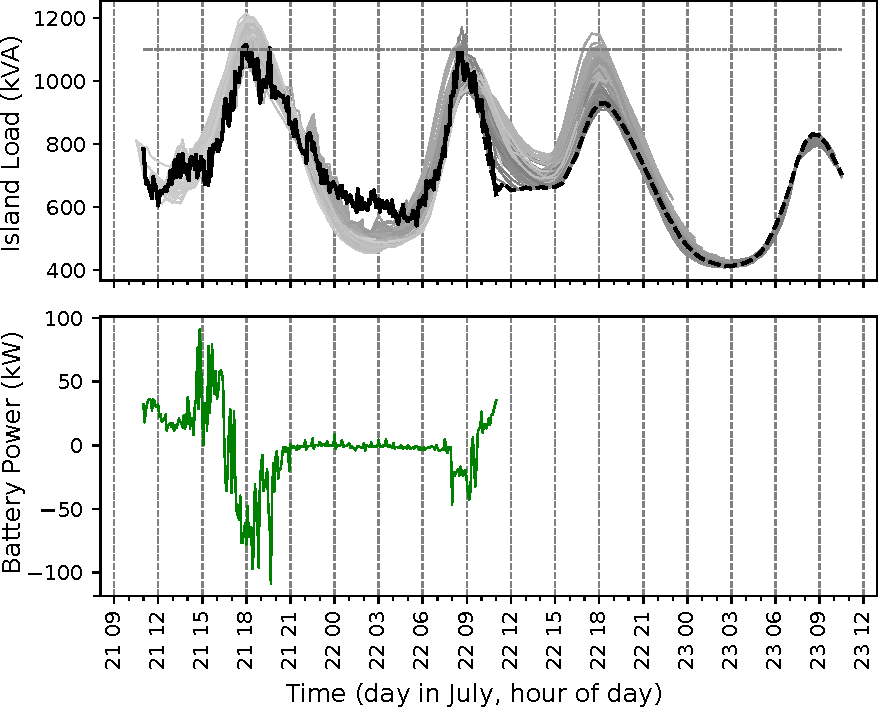
\includegraphics[width=.75\textwidth]{images/bruny_nac.pdf}}
	\caption{Results from the forecasting system's implementation in the CONSORT project.}
	\label{fig:bruny_nac}
\end{figure}


\section{ISO New England}
ISO New England is a regional transmission organization operating in the New England area of the United States.
Data from ISO New England has been used by several papers for evaluating the performance of their load forecasting systems \cite{Ceperic2013}\cite{Chen2010}.
The aim of this section is to compare the proposed forecasting models to the models and methods used by \citet{Ceperic2013}, whose method is discussed in section \ref{SVR}, and \citet{Chen2010}, whose method is discussed in section \ref{litrev-ann}.
A week of load from the ISO New England dataset is shown in figure \ref{fig:week-isone}.

\begin{figure}[htbp]
	\centerline{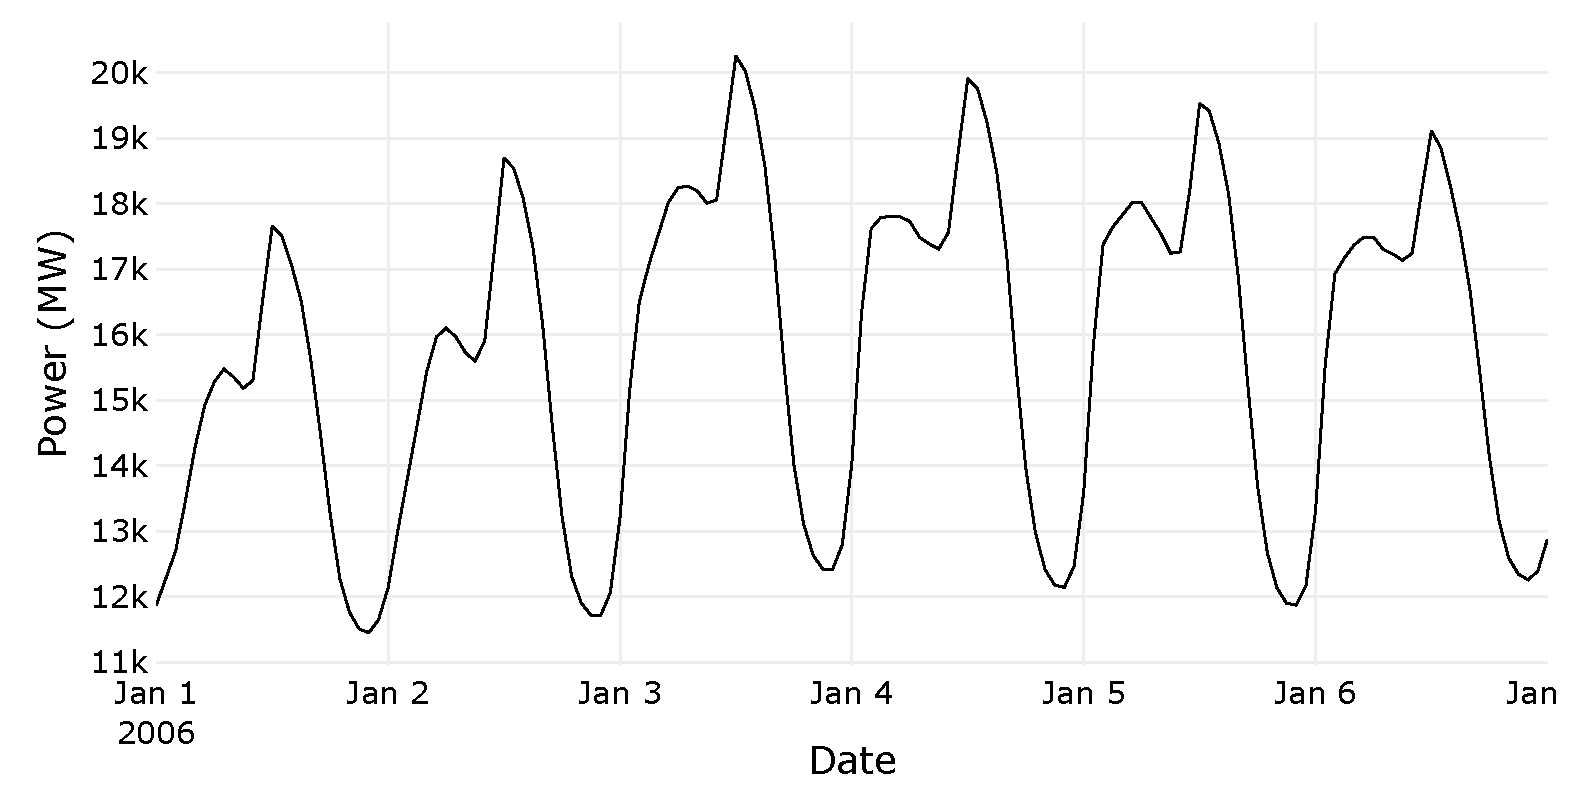
\includegraphics[width=.9\textwidth]{images/week-isone.pdf}}
	\caption{A week of load for ISO New England.}
	\label{fig:week-isone}
\end{figure}

\citet{Ceperic2013} trained their model on data from March 2003 until January 2006 and tested on January 1 2006 to December 31 2006.
Historical electrical load data was obtained from the public ISO New England website \cite{isone}.
Historical temperature was obtained from the National Centers for Environment Information \cite{NOAA} at Concord, New Hampshire, United States (latitude 43.204900 degrees, longitude \mbox{-71.502740 degrees}).
This is different temperature data to that used by \citet{Ceperic2013} as that data could not be accessed.

The following holidays were used, and the same heuristics described in section \ref{simperiod} were applied.
\begin{itemize}
	\item Birthday of Martin Luther King, Jr.;
	\item Washington's Birthday;
	\item Memorial Day;
	\item Independence Day;
	\item Labor Day;
	\item Colombus Day;
	\item Veteran's Day;
	\item Thanksgiving;
	\item Easter; and
	\item Christmas/New Year (Dec 21 through Jan 6).
\end{itemize}

The forecasting was performed identically to the ``hourly long" task described in section \ref{forecasting-tasks}, except with no similar days ($k=0$).
The input matrix $\mX$ was constructed by equation \ref{hourly-long-x}.
\citet{Ceperic2013} turned heuristics about heating and cooling load based on temperature into features for the neural network.
This is generally considered good practice \cite{Zinkevich2018}.
However, as one of the primary aims of this thesis is to develop a practical load forecasting system that does not require significant modifications when forecasting for different feeders, this data was not provided as an input.

The model configurations are the same as that described in table \ref{table:offline-parameters}, and the models were trained for $10^5$ iterations.

\begin{table}[htbp]
	\caption{ISO New England results.}
	\begin{center}
		\begin{tabular}{l|cc}
			%			3.\hline
			\textbf{Model}&\textbf{MAPE (\%)} \\
			\hline
			Transformer no TF            & 2.14 \\ % 151
			S2S                          & 2.15 \\ % 165
			SSA-SVR \cite{Ceperic2013}   & 1.31 \\
			SIWNN \cite{Chen2010}        & 1.71 \\
			ANN \cite{Chen2010}          & 2.03 \\
			Transformer                  & 3.09 \\ % 166
			U. Transformer               & 3.65 \\ % 167
			
		\end{tabular}
		\label{table:iso-results}
	\end{center}
\end{table}

\begin{figure}[htbp]
	\centerline{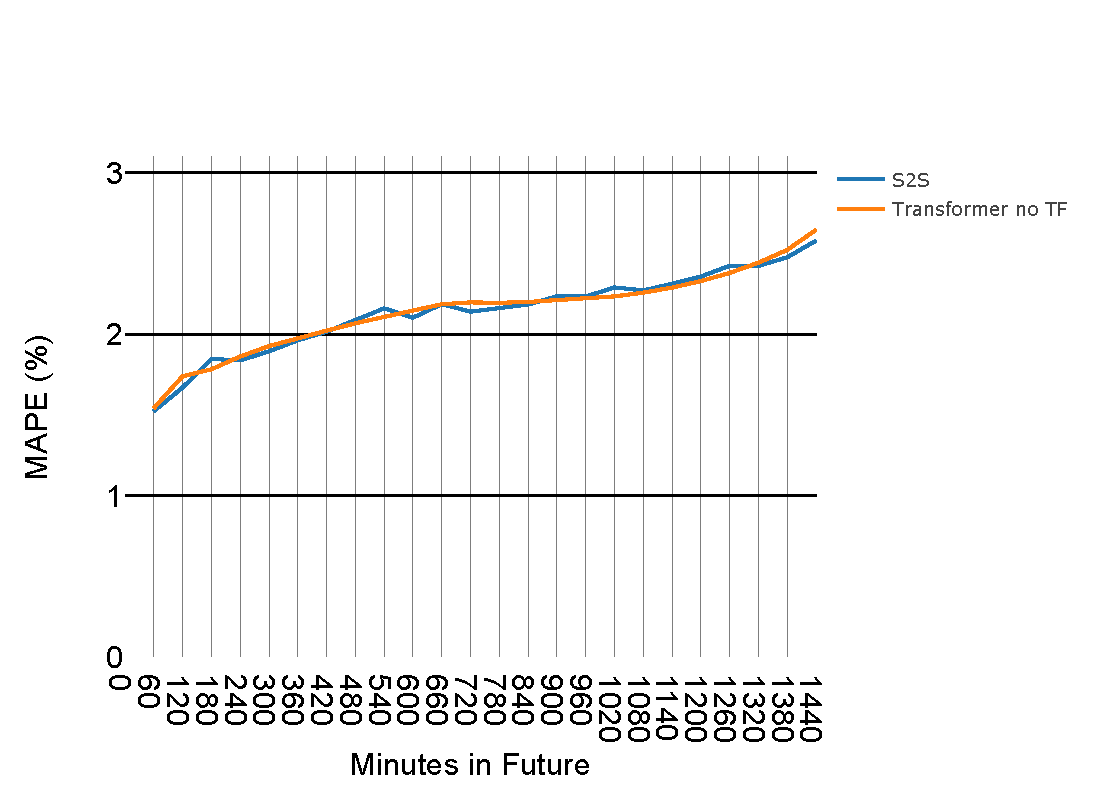
\includegraphics[width=.9\textwidth]{images/iso_mape.pdf}}
	\caption{Mean absolute percentage error of each point in the forecasts for ISO New Egnald, task ``Hourly long".}.
	\label{fig:iso_mape}
\end{figure}

\begin{figure}[htbp]
	\centerline{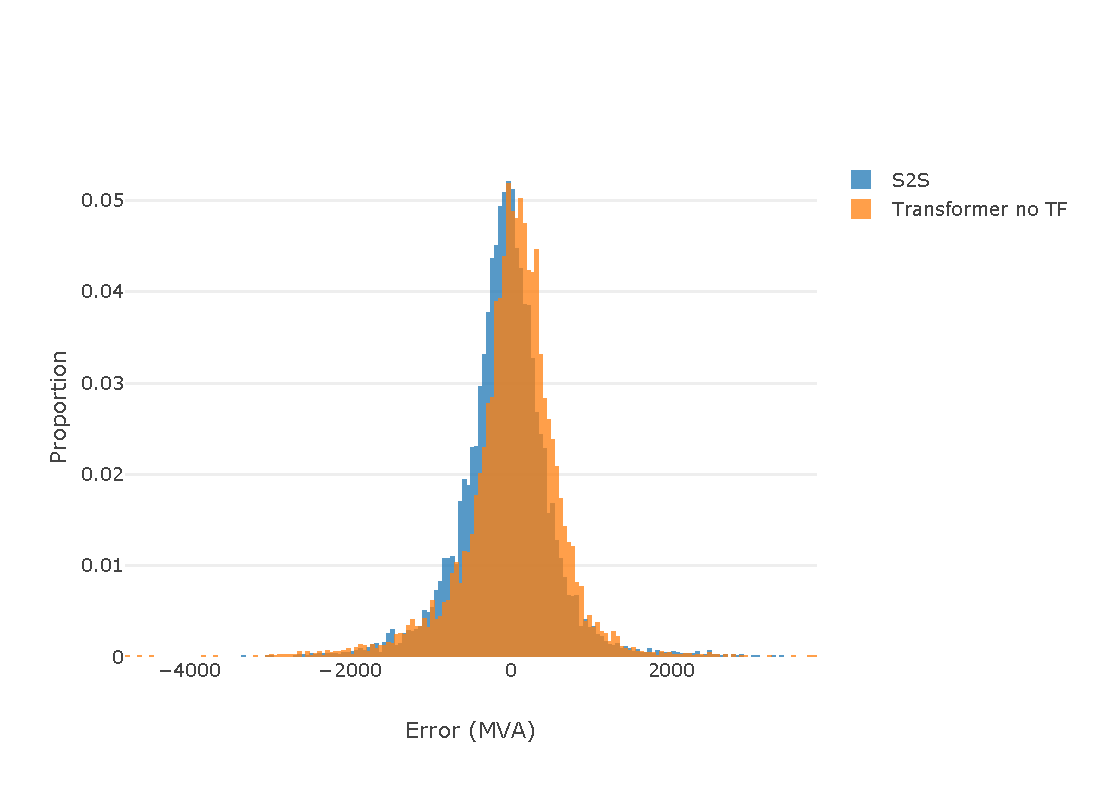
\includegraphics[width=.9\textwidth]{images/iso_hist.pdf}}
	\caption{Distribution of forecast error corresponding to Figure \ref{fig:iso_mape}.}
	\label{fig:iso_hist}
\end{figure}


\section{Discussion}
\chapter{Conclusion}
Four neural-network based models were evaluated for short-term load forecasting: sequence to sequence recurrent neural network, transformer with and without teacher forcing, and universal transformer.
The models were applied to the Bruny Island submarine feeder and to the standard ISO New England dataset.
Metrics assessing the MAPE above 1 MVA and MAPE at first large peak were used to assess the performance of the forecasters on anomalous holiday periods.
The transformer with teacher forcing and universal transformer models did not produce results competitive with the sequence to sequence and transformer without teacher forcing models.

The sequence to sequence model was found to achieve overall good results on the Bruny Island feeder when evaluated on overall MAPE and MAPE above 1 MVA.
The transformer without teacher forcing model was found to achieve the best results on overall MAPE on the Bruny Island feeder, but was somewhat more volatile on the metrics above 1 MVA when compared to the sequence to sequence model. 
The transformer without teacher forcing model also appeared to handle forecasting tasks involving long sequence lengths better than the sequence to sequence model. 
Overall, though, which model is superior on this feeder is not clear and will depend on whether the forecasting is hourly or half-hourly, and whether accuracy overall or accuracy over holiday periods is most important.

A transformer-based model was implemented as part of the Bruny Island CONSORT battery trial and was able to reliably and accurately predict large peaks over anomalous holiday periods.
This was in one instance able to assist the CONSORT project in coordinating the batteries on Bruny Island to avoid using the diesel generator.

The models were additionally evaluated on a standard ISO New England dataset.
When using identical models to those applied on Bruny Island the sequence to sequence and transformer without teacher forcing models were able to achieve a MAPE of 2.15\% compared to other papers of 1.71\% and 1.31\%.

The presented models -- sequence to sequence and transformer without teacher forcing -- are versatile and reliable when used to forecast load with a 24-hour horizon and 30- or 60-minute resolution.
The models are practical to implement and can be applied to feeders ranging from the 1 MVA through 20 GW level with no modifications.
The models can reliably predict anomalous holiday periods given simple inputs describing the holidays and optionally given similar load profiles from the past.

\section{Future research}

\subsubsection{Transfer learning}
OpenAI has had success using transfer learning for natural language processing tasks with the transformer model \cite{radford2018improving}.
Transfer learning could be applied to load forecasting, whereby a single neural network model is first trained to forecast many different feeders, and then this pre-trained model is finally trained to forecast a single feeder.
This could potentially expand the generalization ability of the model, while also likely reducing the amount of training time required when starting from a pre-trained model.

\subsubsection{Monthly and hourly models}
Similar to \citet{Ceperic2013}, different models could be train for every month and every hour.
This introduces 288 models, making the training time potentially quite large, so pre-training or transfer learning could be used to make this more approachable.
This may not work well when considering holiday periods that change yearly, such as Easter which may be in either March or April.

\subsubsection{Multi-task learning}
Multi task learning is the process of using a neural network model to perform multiple tasks simultaneously, and has been shown to improve performance in some tasks \cite{Evgeniou2004}.
This could applied to load forecasting by forecasting multiple feeders simultaneously.
It's intuitive that this might be beneficial, as there are many feeders which exhibit similar patterns -- Bruny Island and St Helens in Tasmania, for example, both experience similar peaks around holiday periods.
This could also allow the forecasting system to be more resilient against poor quality data, as data from one feeder would be used to help forecast others.

\subsubsection{Generic forecaster}
The transformer, and its multi-head self attention, is able to process sequences of long length with no regard for position or order.
This could be used to create a generic forecaster, where the model is supplied with all past data up to the current time when performing forecasts.
A model like this might be able to look over the past data and produce a single forecast that matches the past patterns.
Using multi-head self attention for this would be prohibitively computationally expensive, so localised multi-head attention \cite{Vaswani2017} could be applied, as used by \citet{Song2017}.
If a single model could be made to forecast all feeders this may ultimately be computationally cheaper than using a single model for every feeder.

\subsubsection{Sequence to sequence with attention}
Sequence to sequence models can be augmented with an attention mechanism \cite{luong2015effective} to allow the model to consider all elements of the input simultaneously while producing the output sequence.
This may overcome the tendency of LSTM RNN networks to ``forget" data from early in the input sequence.
Very recently LSTM RNN models have been combined with transformer models \cite{chen2018best}, producing promising results.
Applying combinations of LSTM and attention to load forecasting may produce superior results to either on their own.

\subsubsection{Signal decomposition}
\citet{Chen2010} used wavelet decomposition to decompose input data into low and high frequency components before forecasting the next day's low and high frequency load separately.
\citet{Bedi2018} used empirical mode decomposition to decompose input data into different intrinsic mode functions before applying different LSTM RNNs to each and recombining the results to form a final forecast.
By applying methods such as these it would likely be possible to improve the accuracy of the load forecasting.
However, it may jeopardize the ability for the forecasting models to be applied to different feeders with no modification.


% \chapter{Introduction}\todo[inline]{modify chapter headings as required}

\section{Background to the problem}

Normal `sentence case' is preferred for all headings, don't capitalise each word (e.g.~as above, not ``Background to the Problem").

\subsection{Brief Bib\TeX\ tips}

To illustrate the difference between \verb|\citet| and \verb|\citep|, and how to cite an honours thesis:
\begin{itemize}
  \item \citet{Smith} studied the problem of writing templates, but
  \item many examples of citing honours theses exist in the literature \citep{Smith}.
\end{itemize}
Refer to a standard as follows \citep{ISO3382-2}. With multiple authors make sure you separate each of the author's names with `and' \citep{BookExample}. Note the following features in this reference to \citet{vonKarman}:
\begin{itemize}
  \item multiple authors separated by `and' in the {\tt .bib} file,
  \item special character (\'a)
  \item compound surname needs to be contained in \{\}
  \item use of `DOI' reference (digital object identifier)  
\end{itemize}

More information can be found at \url{http://www.bibtex.org/} and some good examples at \url{https://verbosus.com//bibtex-style-examples.html}.

\subsection{Tables and figures}

Table~\ref{tab:demo} illustrates a simple table, while Figure~\ref{fig:demo} illustrates a figure with subfigures.



\begin{table}[htbp]
  \centering
  \begin{tabular}{ccl}
    \hline
    \textbf{Sample} & \textbf{Maximum recorded} &  \textbf{Failure location} \\
    \textbf{}		& \textbf{load (kN)}		&  \textbf{} \\
    \hline
    $C$    &  197.0  &  Top machined face     \\
    $U_1$  &  199.2  &  Above concrete        \\
    $U_2$  &  221.4  &  Top machined face     \\
    $W_1$  &  199.0  &  Middle machined face  \\
    $W_2$  &  197.0  &  Bottom machined face  \\
    \hline
    \end{tabular}
  \caption{A sample table.}
  \label{tab:demo}
\end{table}

\begin{figure}[htbp]
\centering
	\subfigure[Left subfigure.]{
        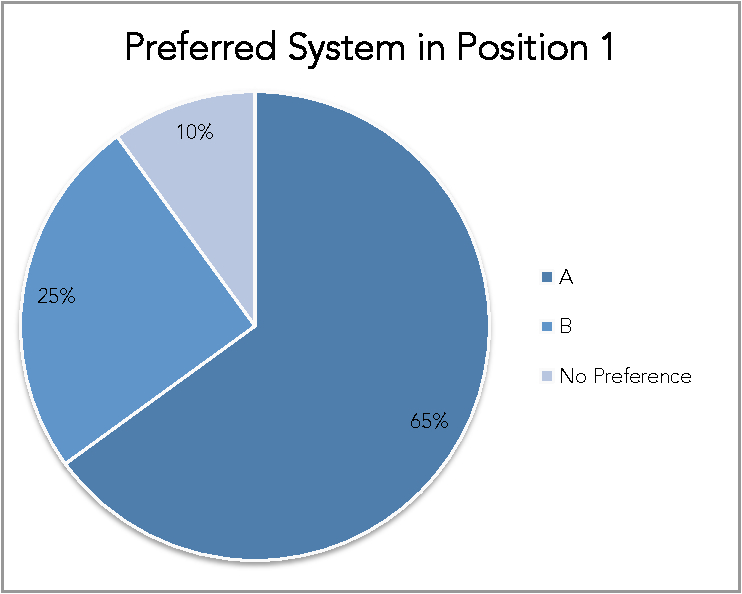
\includegraphics[width=.35\textwidth]{Pos1.pdf}
        \label{fig:Pos1}}
 \quad\quad
	\subfigure[Right subfigure.]{
        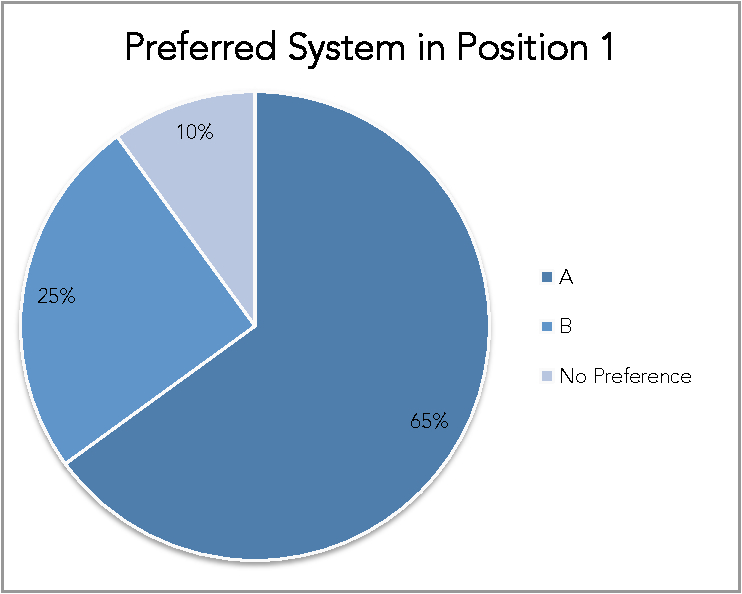
\includegraphics[width=.35\textwidth]{Pos1.pdf}
        \label{fig:Pos2}}
   \caption{A sample two part figure using the {\tt subfigure} package.}
  \label{fig:demo}
\end{figure}


\section{Problem statement}

\section{Project scope}

% \chapter{Background theory}
   \section{Chapter intro}
   \section{Chapter body}
   \section{Chapter summary}

\chapter{Literature review}
   \section{Chapter intro}
   \section{Chapter body}
   \section{Chapter summary}

\chapter{Experimental method}
   \section{Chapter intro}
   \section{Chapter body}
   \section{Chapter summary}

\chapter{Results}
   \section{Chapter intro}
   \section{Chapter body}
   \section{Chapter summary}

\chapter{Discussion}
   \section{Chapter intro}
   \section{Chapter body}
   \section{Chapter summary}

\chapter{Conclusions and further work}
   \section{Summary of findings}
   \section{Limitations and recommendations}
   \section{Suggestions for further work}

% =========================================================================
%                        References/Bibliography
% Note that you must use a style that is compatible with the natbib package
% (e.g. plainnat or newapa) or remove "\usepackage{natbib}" from preamble.
% =========================================================================
\bibliographystyle{IEEEtranN}   % choose a style here
\cleardoublepage \phantomsection \addcontentsline{toc}{chapter}{\bibname}  % This adds it to the table of contents with the right page numbering
\bibliography{lf-thesis}             % Your 'bib' file

% =========================================================================
%                        Appendices 
% =========================================================================
% \appendix                 % This changes numbering from 1, 2 etc. to A, B etc.
\cleardoublepage          % these lines add it to the table of contents
\phantomsection
\addcontentsline{toc}{chapter}{Appendices}

%===================================
%       EDIT BELOW THIS LINE
%===================================

% The first appendix
\chapter{Extra stuff}

% The second appendix
\chapter{More extras}

% =========================================================================
%                        Back matter (if required, otherwise delete) 
% =========================================================================
%\backmatter

\end{document}